% =====================================================================
% Prevalidación documental para la residencia definitiva (SERMIG)
% Autora: Trina Isabel Palacios Hernández
% Versión 13. Compila con XeLaTeX (recomendado) o pdfLaTeX.
% En Overleaf: Menu > Compiler > XeLaTeX.
% Requiere en la misma carpeta: fig_evaluaciones.pdf, fig_derivacion_pais.pdf y
% tabla_condiciones.tex, tabla_deteccion.tex y tabla_linea_base.tex (generados por scripts/figuras.py de la maqueta).
% Los diagramas son TikZ.
% =====================================================================
\documentclass[11pt,a4paper]{article}

\usepackage{iftex}
\ifXeTeX
  \usepackage{fontspec}
  \usepackage{polyglossia}
  \setmainlanguage{spanish}
  \setotherlanguage{english}
\else
  \usepackage[utf8]{inputenc}
  \usepackage[T1]{fontenc}
  \usepackage{lmodern}
  \usepackage[english,spanish,es-noshorthands,es-tabla]{babel}
\fi

\usepackage[margin=2.5cm]{geometry}
\usepackage{graphicx}
\usepackage{booktabs}
\usepackage{tabularx}
\usepackage{array}
\usepackage{enumitem}
\usepackage{caption}
\usepackage{float}
\usepackage{listings}
\usepackage{etoolbox}
\usepackage{catchfile}
\usepackage{tikz}
\usetikzlibrary{positioning,shapes.geometric,arrows.meta,fit,backgrounds,calc}
\usepackage[hidelinks]{hyperref}
\usepackage{xurl}

\ifXeTeX
  \gappto\captionsspanish{\renewcommand{\tablename}{Tabla}\renewcommand{\listtablename}{Índice de tablas}}
\fi

\captionsetup{font=small,labelfont=bf}
\setlist{itemsep=2pt,topsep=4pt}
\newcolumntype{L}{>{\raggedright\arraybackslash}X}
\newcolumntype{C}{>{\centering\arraybackslash}X}
\renewcommand{\arraystretch}{1.25}
\setlength{\emergencystretch}{3em}

\lstset{basicstyle=\ttfamily\scriptsize,frame=single,columns=fullflexible,breaklines=true,xleftmargin=2mm,xrightmargin=2mm,framesep=2mm,aboveskip=6pt,belowskip=6pt,extendedchars=true,
  literate={á}{{\'a}}1 {é}{{\'e}}1 {í}{{\'i}}1 {ó}{{\'o}}1 {ú}{{\'u}}1 {ñ}{{\~n}}1 {Ñ}{{\~N}}1 {Í}{{\'I}}1 {Ó}{{\'O}}1}
\AtBeginDocument{\renewcommand{\lstlistingname}{Listado}}
% Flotantes: más contenido por página y páginas de flotantes alineadas arriba
\renewcommand{\topfraction}{0.85}\renewcommand{\bottomfraction}{0.6}
\renewcommand{\textfraction}{0.1}\renewcommand{\floatpagefraction}{0.7}
\setcounter{topnumber}{3}\setcounter{totalnumber}{5}
\makeatletter\setlength{\@fptop}{0pt}\setlength{\@fpbot}{0pt plus 1fil}\makeatother

\tikzset{
  proc/.style={rectangle,rounded corners=2pt,draw=black!70,fill=white,align=center,font=\scriptsize,minimum height=8mm,text width=24mm,inner sep=2pt},
  dec/.style={diamond,draw=black!70,fill=white,align=center,font=\scriptsize,aspect=1.8,inner sep=1pt,text width=15mm},
  hot/.style={proc,draw=red!70!black,fill=red!8,line width=0.8pt},
  auto/.style={proc,draw=blue!60!black,fill=blue!6},
  hum/.style={proc,draw=green!40!black,fill=green!8},
  ev/.style={circle,draw=black!70,minimum size=5mm,inner sep=0pt,font=\scriptsize},
  arr/.style={-{Stealth[length=2mm]},draw=black!70},
  lane/.style={draw=black!40,fill=black!3},
  lbl/.style={font=\scriptsize\bfseries,rotate=90,anchor=south},
  note/.style={font=\tiny\itshape,text=red!60!black,align=center},
  lab/.style={font=\tiny,fill=white,inner sep=1pt},
  svc/.style={rectangle,rounded corners=2pt,draw=black!70,fill=white,align=center,font=\scriptsize,minimum height=9mm,text width=23mm,inner sep=2pt},
  grp/.style={draw=black!50,dashed,rounded corners=4pt,inner sep=3mm},
  grplbl/.style={font=\scriptsize\bfseries,anchor=south west},
}

\title{\textbf{Prevalidación documental mediante interoperabilidad, firma electrónica y reconocimiento óptico de caracteres para la residencia definitiva en el Servicio Nacional de Migraciones de Chile: arquitectura y maqueta funcional}}
\author{Trina Isabel Palacios Hernández\\[2pt]
\small Magíster en Ingeniería Informática (c), Universidad Bernardo O'Higgins, Santiago, Chile\\
\small \texttt{issabelpalacios@gmail.com}}
\date{Octubre de 2026}

\begin{document}
\maketitle

% ---------------------------------------------------------------------
\begin{abstract}
\noindent
Las solicitudes de residencia definitiva en Chile enfrentan demoras prolongadas y una alta carga de revisión documental en el Servicio Nacional de Migraciones. Con el enfoque de ciencia del diseño, este trabajo se pregunta cómo diseñar un sistema de prevalidación documental que reduzca esa carga sin automatizar decisiones, y desagrega la pregunta en tres: qué documentos y qué etapas concentran la revisión, qué arquitectura permite verificar cada documento por la vía más confiable, y cómo demostrar el diseño y evaluarlo. El diagnóstico, basado en fuentes oficiales, identifica dos etapas de revisión manual y clasifica los documentos según su origen. La solución verifica los documentos públicos chilenos con su emisor, valida por su firma los firmados electrónicamente y lee solo los demás con reconocimiento óptico de caracteres (OCR) y reglas. El sistema no decide: advierte y, ante una lectura dudosa, deriva a revisión humana. La arquitectura mantiene los datos en Chile y hace intercambiable el motor OCR. Una maqueta funcional en Python demuestra las tres vías con documentos ficticios. Al probarla surgió un problema metodológico: los documentos de prueba parecidos a los de desarrollo daban una imagen optimista, que no se sostuvo ante documentos con diagramaciones nuevas generados después de congelar el código. El trabajo propone cómo resolverlo: criterios fijados antes de evaluar, corpus independientes y documentos reales, un estudio de tiempos con funcionarios y un piloto. El ahorro de tiempo y el desempeño con documentos reales quedan por medir.

\medskip
\noindent\textbf{Palabras clave:} prevalidación documental, OCR, interoperabilidad, firma electrónica, ciencia del diseño, migración.
\end{abstract}

\begin{otherlanguage}{english}
\begin{abstract}
\noindent
Permanent residence applications in Chile face long delays and a heavy document review burden at the National Migration Service. Following the design science research approach, this work asks how to design a document pre-validation system that reduces that burden without automating decisions, and breaks it down into three specific questions: which documents and stages concentrate the review, which architecture allows each document to be verified through the most reliable route, and how to demonstrate and evaluate the design. The diagnosis, based on official sources, identifies two manual review stages and classifies documents by origin. The solution verifies Chilean public documents with their issuer, validates electronically signed documents through their signature, and reads only the rest with optical character recognition (OCR) and rules. The system does not decide: it warns and, whenever a reading is uncertain, refers the document to human review. The architecture keeps data in Chile and makes the OCR engine interchangeable. A functional mock-up in Python demonstrates the three routes with fictitious documents. Testing it revealed a methodological problem: test documents similar to the development ones gave an optimistic picture that did not hold for documents with new layouts generated after the code freeze. The work proposes a solution: criteria fixed before evaluating, independent corpora and real documents, a time study with officials and a pilot. Time savings and performance on real documents remain to be measured.

\medskip
\noindent\textbf{Keywords:} document pre-validation, OCR, interoperability, electronic signature, design science, migration.
\end{abstract}
\end{otherlanguage}

% ---------------------------------------------------------------------
\section{Introducción}
\label{sec:intro}

Chile ha sido protagonista de un proceso migratorio sostenido: según la última estimación oficial, más de 1,9 millones de personas extranjeras residían en el país a fines de 2023 \cite{ine2024}. Esta realidad ha generado una fuerte presión institucional, particularmente en los trámites de residencia definitiva, donde las demoras y la sobrecarga administrativa afectan tanto a las personas solicitantes como al personal del Servicio.

Este trabajo propone la arquitectura de un sistema de prevalidación de los documentos que acompañan las solicitudes de residencia definitiva y la demuestra con una maqueta funcional. Una precisión conceptual guía todo el documento: el OCR \emph{extrae} información, pero no determina si un documento es auténtico. Por ello, la solución automatiza la lectura y los controles formales, privilegia la verificación con el emisor y deja siempre la decisión en manos de un funcionario.

\subsection{Problemática}
\label{sec:problema}
En 2024 el SERMIG acogió a trámite 136.848 solicitudes de residencia definitiva y otorgó 133.726 permisos, la mayor cifra de otorgamientos de la última década \cite{sermig2025}. A febrero de 2025, el Servicio informó haber resuelto 382.743 de las 386.024 solicitudes de residencia definitiva que estaban pendientes desde antes de diciembre de 2022 \cite{sermigavances}. No se publican, en cambio, el número actual de solicitudes pendientes ni los tiempos de tramitación de la población adulta.

La Ley N.º 19.880 establece que un procedimiento administrativo no puede exceder de seis meses desde su inicio hasta la decisión final, salvo caso fortuito o fuerza mayor \cite{ley19880}. El único dato público desagregado corresponde a niños, niñas y adolescentes: según la Defensoría de la Niñez, entre 2022 y 2024 la tramitación de sus residencias definitivas tardó en promedio 770 días, con promedios anuales de 819 días en 2022, 868 en 2023 y 645 en 2024 \cite{defensoria2026}. La cifra de 770 días es el promedio del período informado por la Defensoría, que no coincide con el promedio simple de los tres promedios anuales. Las demoras han motivado numerosos recursos judiciales de personas que solicitan que el Servicio se pronuncie \cite{latercera2023}.

Este trabajo aborda una parte acotada del problema: la revisión de los documentos que acompañan cada solicitud. El análisis del proceso (sección~\ref{sec:diagnostico}) identifica dos puntos donde esa revisión genera carga y demora: la revisión formal al acoger la solicitud, que cuando detecta un documento faltante o vencido emite un requerimiento con hasta 60 días corridos de plazo para responder \cite{sermigrd}; y la revisión de fondo, en la que los funcionarios leen y verifican documentos heterogéneos, incluida su autenticidad. Un caso resuelto por la Corte Suprema muestra que la adulteración de certificados de antecedentes es un riesgo real: el Servicio constató que el código QR del certificado presentado correspondía a otra persona \cite{cs2026}.

Este trabajo no sostiene que la revisión documental sea la única causa de las demoras: también influyen la dotación de personal, el volumen acumulado y las consultas a otros organismos. Su peso relativo no puede cuantificarse con datos públicos y se aborda en el protocolo de evaluación propuesto (sección~\ref{sec:pendiente}). Más aún, que la revisión documental sea un cuello de botella es una inferencia a partir del flujo publicado, no un dato: el Servicio informa haber resuelto el 99\,\% del rezago anterior a diciembre de 2022 y no publica tiempos por etapa. La relevancia del problema se apoya en lo que sí está documentado: los requerimientos de antecedentes, que otorgan hasta 60 días para responder \cite{sermigrd}, y un caso de certificado adulterado que llegó a la Corte Suprema \cite{cs2026}.

\subsection{Justificación}
\textbf{Técnico.} Las tecnologías de OCR permiten automatizar la extracción de datos de documentos impresos \cite{hegghammer2022}, y buena parte de los documentos chilenos exigidos ya cuenta con verificación electrónica, lo que permite combinar ambas estrategias.

\textbf{Social.} Una alerta inmediata a la persona solicitante (por ejemplo, ``su certificado tiene más de 60 días de emitido'') permite corregir en el momento un problema que hoy se conoce solo al recibir un requerimiento, semanas o meses después. Por la misma razón, una alerta injustificada tiene un costo para la persona, que puede reemplazar sin necesidad un documento válido; por eso este trabajo trata las alertas injustificadas como un error de primer orden.

\textbf{Normativo.} La Ley N.º 21.180 exige que los procedimientos se tramiten de forma electrónica y que los órganos del Estado intercambien información por medios interoperables \cite{ley21180}. La Ley N.º 21.719 exigirá estándares de licitud, finalidad, seguridad y transparencia, incluidas reglas sobre decisiones automatizadas \cite{ley21719}.

\subsection{Preguntas de investigación}
\label{sec:pregunta}
La investigación se organiza en torno a una pregunta general:

\begin{quote}
\textbf{PG.} \emph{¿Cómo diseñar un sistema de prevalidación documental para la residencia definitiva que reduzca la carga de revisión documental del Servicio Nacional de Migraciones, combinando interoperabilidad, firma electrónica y OCR, sin automatizar decisiones ni dar por conforme en silencio un documento con problemas?}
\end{quote}

La pregunta general se desagrega en tres preguntas específicas, cada una con la solución que propone este trabajo:
\begin{description}[leftmargin=1.2cm,style=nextline]
  \item[PE1.] \emph{¿Qué documentos exige la residencia definitiva, cuál es su origen y en qué etapas del proceso su revisión genera carga y demora?} Solución: un diagnóstico del proceso que clasifica los documentos por su origen y asigna a cada grupo una vía de verificación (sección~\ref{sec:diagnostico}).
  \item[PE2.] \emph{¿Qué arquitectura, reglas y principios de diseño permiten verificar cada documento por la vía más confiable y derivar a revisión humana lo dudoso, dentro del marco normativo y ético aplicable?} Solución: requerimientos, un flujo de prevalidación, reglas configurables, una arquitectura independiente del proveedor, tres principios de diseño y la contrastación normativa y ética del diseño (secciones~\ref{sec:diseno} y \ref{sec:etica}).
  \item[PE3.] \emph{¿Cómo demostrar la factibilidad del diseño con una maqueta funcional, qué problemas metodológicos aparecen al probarla y cómo deben resolverse para evaluar el sistema antes de adoptarlo?} Solución: una maqueta que implementa las tres vías, el análisis de los problemas metodológicos observados y un protocolo de evaluación con documentos y funcionarios reales (secciones~\ref{sec:implementacion} a \ref{sec:pendiente}).
\end{description}

Las preguntas se limitan deliberadamente al diseño y a su factibilidad técnica. Si el sistema reduce o no la revisión manual depende de cuántos documentos reales logre leer con confianza y del tiempo que ahorre a los funcionarios, lo que exige una evaluación con documentos y funcionarios reales que este trabajo define, pero no ejecuta (sección~\ref{sec:pendiente}). Por ello, la maqueta se prueba con documentos ficticios para demostrar el diseño y aprender cómo evaluarlo, no para certificar su desempeño. Las pruebas realizadas y sus cifras se documentan en el Anexo~\ref{sec:anexo}.

\subsection{Objetivos}
\paragraph{Objetivo general.} Proponer y demostrar, mediante una arquitectura y una maqueta funcional, un sistema de prevalidación documental basado en interoperabilidad, firma electrónica y reconocimiento óptico de caracteres, que reduzca la carga de revisión documental de la residencia definitiva en el Servicio Nacional de Migraciones de Chile sin automatizar decisiones.

\paragraph{Objetivos específicos.}
\begin{enumerate}[label=\textbf{OE\arabic*.},leftmargin=*]
  \item Analizar el proceso actual de revisión documental de la residencia definitiva, identificando los documentos exigidos, su origen y las etapas que concentran la carga y la demora (PE1).
  \item Diseñar la arquitectura, los requerimientos, las reglas de prevalidación y los principios de diseño del sistema, y contrastarlos con el marco normativo y ético aplicable (PE2).
  \item Construir una maqueta funcional que demuestre el diseño, identificar los problemas metodológicos que aparecen al probarla y proponer un protocolo para evaluar el sistema con documentos y funcionarios reales, incluido un modelo de costos y de horas liberadas (PE3).
\end{enumerate}

\subsection{Alcance}
El trabajo comprende el análisis del proceso a partir de fuentes oficiales, el diseño del sistema, una maqueta funcional probada con documentos ficticios, el análisis de los problemas metodológicos observados, un protocolo de evaluación, un modelo de costos y de horas con supuestos explícitos y la contrastación normativa y ética. Quedan fuera de su alcance:
\begin{itemize}
  \item la medición del desempeño del sistema con criterios de aceptación, que se define en el protocolo propuesto;
  \item un sistema productivo, integraciones reales con el SERMIG u otros organismos y el uso de documentos de personas reales;
  \item la verificación forense de autenticidad, la biometría y la traducción automática;
  \item la ejecución de la maqueta con motores OCR en la nube, cuyos adaptadores están implementados, y
  \item la medición del tiempo ahorrado a los funcionarios y la cuantificación monetaria del ahorro y del costo de implementación.
\end{itemize}

\subsection{Contribución}
En la tipología de Gregor y Hevner \cite{gregor2013}, este trabajo hace una contribución de \emph{exaptación}: soluciones conocidas, como la verificación con el emisor, el OCR y la clasificación con opción de rechazo, se combinan y se extienden a un problema en que no se habían aplicado juntas, la prevalidación documental migratoria. Tiene tres componentes: (1) un artefacto de diseño (flujos, arquitectura, requerimientos y reglas); (2) una maqueta funcional de código abierto que lo implementa; y (3) tres principios de diseño (sección~\ref{sec:principios}). Además, documenta un problema metodológico que surge al probar este tipo de sistemas y propone un protocolo para evaluarlos.

% ---------------------------------------------------------------------
\section{Marco teórico y estado del arte}
\label{sec:marco}

\subsection{Transformación digital e inteligencia artificial en el sector público}
Según la OCDE \cite{ocde2020}, los gobiernos deben avanzar hacia procesos digitales, interoperables y centrados en el ciudadano. El principio de ``solo una vez'' (\emph{once-only}) propone que las personas no entreguen al Estado datos que este ya tiene \cite{krimmer2017}; en Chile, la Ley N.º 21.180 apunta en ese sentido \cite{ley21180}. La literatura sobre inteligencia artificial en el sector público identifica beneficios de eficiencia y desafíos de gobernanza, rendición de cuentas y aceptación \cite{wirtz2019}. Un informe para la Administrative Conference of the United States documentó 157 casos de uso de inteligencia artificial en 64 agencias federales, entre ellos herramientas de apoyo a la adjudicación de casos, y advirtió sobre sus riesgos de rendición de cuentas \cite{engstrom2020}.

\subsection{Reconocimiento óptico de caracteres y procesamiento inteligente de documentos}
El OCR convierte imágenes con texto en texto digital. Tesseract es el motor de código abierto más difundido \cite{smith2007}; desde su versión 4 incorpora reconocimiento basado en redes neuronales recurrentes. Las soluciones actuales identifican además pares clave-valor y tablas, lo que se conoce como procesamiento inteligente de documentos \cite{cui2021}; modelos multimodales como LayoutLMv3 combinan texto, imagen y posición \cite{huang2022}. Desde la práctica industrial, Cutting y Cutting-Decelle \cite{cutting2021} señalan que la integración con los procesos de negocio y los documentos poco estructurados siguen siendo los principales desafíos. Este último punto es central para este trabajo: ubicar un campo por su etiqueta funciona mientras la diagramación sea la esperada, y las pruebas de la maqueta (sección~\ref{sec:metodologico}) muestran qué ocurre cuando no lo es.

Hegghammer \cite{hegghammer2022} comparó Tesseract, Amazon Textract y Google Document AI sobre más de 18.000 documentos en inglés y árabe con ruido artificial: Document AI obtuvo los mejores resultados, y los servicios en la nube superaron ampliamente a Tesseract en imágenes degradadas. El estudio no evaluó español ni francés, por lo que la elección del motor debe basarse en pruebas con documentos representativos.

En los últimos años, los modelos multimodales de lenguaje y visión se han incorporado a la extracción documental. Este trabajo no los evalúa por cuatro razones vinculadas a su diseño: no entregan, en general, una confianza por campo calibrable como la que exigía el diseño inicial del principio 3; pueden generar valores plausibles que no están en el documento; las evaluaciones públicas muestran que leen de forma irregular el texto sin significado léxico, manuscrito o en varios idiomas \cite{ocrbench2024}, justamente el caso de números de documento, códigos y nombres; y su uso implica transferir documentos completos a un proveedor externo. El adaptador OCR de la maqueta permite incorporarlos y compararlos en trabajos futuros.

\subsection{Pasaportes y zona de lectura mecánica}
Los pasaportes emitidos conforme al Doc 9303 de la Organización de Aviación Civil Internacional (OACI) incluyen una zona de lectura mecánica (MRZ) de dos líneas de 44 caracteres, impresa en la tipografía OCR-B, con cinco dígitos de control: número de documento, fecha de nacimiento, fecha de vencimiento, número personal y dígito compuesto \cite{icao9303}. Los nombres se transcriben sin tildes, se truncan cuando no caben en los 39 caracteres disponibles y no están protegidos por dígitos de control, de modo que un dígito de control válido no garantiza que el nombre se haya leído bien. La extracción automática de la MRZ es un problema estudiado: Liu et al. \cite{liu2021} reportan una detección del 100\,\% y un F1 de reconocimiento de caracteres de 98,36\,\% con redes convolucionales. Existen además conjuntos públicos de documentos de identidad ficticios para evaluar estos sistemas, como MIDV-2020 \cite{bulatov2022}; este trabajo no lo usó, y el protocolo propuesto lo incluye como el paso más directo para contrastar las pruebas sintéticas con diagramaciones reales (sección~\ref{sec:pendiente}).

\subsection{Extracción de datos frente a verificación de autenticidad}
La extracción y prevalidación consiste en leer datos y comprobar reglas formales; la verificación de autenticidad consiste en determinar si un documento fue emitido por quien dice y si fue alterado. Esta última es un problema abierto y cada vez más complejo: la IA generativa permite fabricar documentos de alta fidelidad, y los métodos de detección muestran una brecha persistente entre su desempeño en pruebas y en condiciones reales \cite{das2026}. Por ello, la propuesta no atribuye al OCR capacidad de detectar falsificaciones y privilegia la verificación con el emisor y la firma electrónica.

\subsection{Firma electrónica avanzada}
La Ley N.º 19.799 regula los documentos electrónicos y la firma electrónica: los actos suscritos con firma electrónica producen los mismos efectos que los celebrados por escrito, y la firma electrónica avanzada, certificada por un prestador acreditado, se exige para los instrumentos públicos electrónicos y les otorga mayor valor probatorio \cite{ley19799}. Técnicamente, validar una firma en un documento PDF implica comprobar que el contenido firmado no fue modificado (integridad) y que el certificado del firmante proviene de una cadena de certificación confiable (confianza). Hay dos aspectos adicionales que una validación ingenua omite. Primero, el formato PDF admite \emph{actualizaciones incrementales}: se puede agregar contenido después de la firma sin invalidarla criptográficamente, porque la firma cubre solo la revisión firmada \cite{iso32000}; por eso el validador debe verificar también qué cambió después de firmar. Segundo, una firma válida solo acredita a quien firmó: si el documento declara un empleador, debe comprobarse que el firmante sea ese empleador o actúe en su nombre, lo que no es evidente cuando firma una persona natural, como un representante legal o un encargado de remuneraciones, cuyo RUT no es el de la empresa. Una validación completa verifica además la revocación del certificado y el sello de tiempo.

\subsection{Trabajos relacionados en migración}
El antecedente más cercano es el sistema de analítica avanzada de Inmigración, Refugiados y Ciudadanía de Canadá (IRCC), que clasifica las solicitudes de visa de residente temporal y agiliza las rutinarias. Según la agencia, el sistema nunca rechaza ni recomienda rechazar solicitudes, y toda negativa la decide un funcionario \cite{ircc2022}. Aun con esas salvaguardas, Das et al. \cite{dasd2026} documentan asimetrías de rendición de cuentas: los solicitantes no acceden a la lógica de decisión y viven la espera con incertidumbre. Molnar y Gill \cite{molnar2018} advierten que estos sistemas pueden reproducir sesgos si no existen supervisión, transparencia y vías de impugnación, y Canadá exige evaluaciones de impacto algorítmico e intervención humana proporcional al riesgo \cite{canada2019}. Los algoritmos en migración se han aplicado también a la asignación geográfica de refugiados para mejorar su integración \cite{bansak2018}.

Otras tres líneas de trabajo resuelven partes del problema. Los sistemas de verificación de identidad a distancia (eKYC) combinan la lectura de documentos de identidad, la MRZ y la biometría para incorporar clientes \cite{das2026}; verifican una identidad, no la vigencia ni la coherencia de un expediente con documentos heterogéneos. Las infraestructuras de intercambio de datos entre organismos, como X-Road en Estonia \cite{xroad}, y el proyecto europeo TOOP, que llevó el principio de ``solo una vez'' al intercambio entre países \cite{toop2021}, suponen que el dato existe en un registro accesible, lo que no ocurre con los certificados extranjeros ni con los documentos privados. Por último, los sistemas de clasificación de solicitudes, como el de Canadá, deciden prioridades, no revisan documentos. En las fuentes revisadas no se identificaron trabajos sobre prevalidación de expedientes migratorios que combinen verificación con el emisor, validación de firma y lectura con abstención. Esa combinación, aplicada a documentos extranjeros que no están en registros accesibles, justifica clasificar la contribución como exaptación. La revisión no fue sistemática, lo que constituye una limitación.

\subsection{Opción de rechazo y sesgo de automatización}
Chow \cite{chow1970} formalizó el compromiso entre error y rechazo de un clasificador: abstenerse en los casos dudosos reduce los errores a costa de dejar casos sin resolver. La clasificación selectiva \cite{geifman2017} extiende la idea a las redes neuronales y la expresa como un compromiso entre riesgo y cobertura. El principio de derivar ante la duda aplica ese esquema: una derivación es una abstención que resuelve un funcionario, y la proporción de documentos no derivados es la cobertura. La literatura sobre automatización advierte, a la vez, que las personas tienden a confiar en exceso en las ayudas automatizadas, por complacencia o por sesgo de automatización \cite{parasuraman2010}. En el sector público, un estudio experimental no encontró un sesgo de automatización general, pero sí adherencia selectiva: los decisores siguieron más el consejo algorítmico cuando coincidía con estereotipos sobre grupos minoritarios \cite{alonbarkat2023}, un riesgo directo en decisiones migratorias. Por eso un sistema que solo advierte no elimina el riesgo de decisiones automatizadas de hecho, y debe medirse cómo usan los funcionarios sus alertas.

\subsection{Marco normativo}

\paragraph{Marco migratorio.} La Ley N.º 21.325 de Migración y Extranjería regula la residencia definitiva. Su artículo 78 la reserva a residentes temporales cuyo permiso los habilite y que cumplan los requisitos de la ley, su reglamento y el decreto de subcategorías; su artículo 88 obliga a rechazar mediante resolución fundada las solicitudes que no los cumplan \cite{ley21325}. El Decreto N.º 177 de 2022, que establece las subcategorías migratorias de residencia temporal, exige en su artículo 11, letra b), que las personas mayores de edad presenten el certificado de antecedentes del país de origen o de aquel en que hayan residido en los últimos cinco años \cite{decreto177}; la Corte Suprema aplicó esa exigencia al revisar el rechazo de una residencia definitiva \cite{cs2026}.

\paragraph{Autenticación de documentos extranjeros.} Los documentos públicos de países parte de la Convención de La Haya de 1961 se autentican con una apostilla; los de países que no son parte requieren legalización consular. Chile, Venezuela, Perú, Colombia y Bolivia son parte de la Convención; Haití no lo es \cite{hcch2026}. Por ello la regla de autenticación depende del país emisor.

\paragraph{Procedimiento administrativo y gobierno digital.} La Ley N.º 19.880 regula los procedimientos administrativos \cite{ley19880}. La Ley N.º 21.180 la modifica para que los procedimientos se tramiten en expediente electrónico y para que los órganos del Estado obtengan por medios interoperables los documentos que ya obran en poder de otros organismos \cite{ley21180}.

\paragraph{Protección de datos personales.} La Ley N.º 21.719, publicada el 13 de diciembre de 2024 y originada en los boletines refundidos N.º 11.092-07 y 11.144-07, modifica la Ley N.º 19.628 \cite{ley19628} y crea la Agencia de Protección de Datos Personales \cite{ley21719,bcn21719}. Su entrada en vigencia está fijada para el 1 de diciembre de 2026. El Boletín N.º 18.623-07, presentado por mensaje presidencial fechado el 31 de agosto de 2026, propone postergarla hasta el 1 de diciembre de 2027 \cite{cariola2026,parlamento2026}. En octubre de 2026 la Comisión de Constitución del Senado lo aprobó en general, junto con el Boletín N.º 18.060-07, y se discutió también una postergación parcial \cite{jdf2026}. A la fecha de este trabajo, la ley sigue fijada para regir el 1 de diciembre de 2026. Para esta propuesta son relevantes las reglas sobre tratamiento por órganos públicos, la transferencia internacional de datos y el artículo 8 bis de la Ley N.º 19.628, introducido por la Ley N.º 21.719, sobre decisiones basadas únicamente en tratamiento automatizado \cite{ley21719}.

\paragraph{Ciberseguridad y transparencia.} La Ley N.º 21.663, Marco de Ciberseguridad, impone obligaciones de gestión de riesgos y de reporte de incidentes a los órganos de la Administración del Estado \cite{ley21663}. La Ley N.º 20.285 permite solicitar al Servicio información no publicada \cite{ley20285}. La norma ISO/IEC 27001:2022 \cite{iso27001} ofrece los controles de referencia usados en la contrastación normativa (sección~\ref{sec:cumplimiento}).

\subsection{Ética en decisiones automatizadas}
La UNESCO ha propuesto principios para que la inteligencia artificial se desarrolle con equidad, transparencia y rendición de cuentas \cite{unesco2021}. Busuioc advierte que los algoritmos en el sector público plantean un problema de rendición de cuentas: los funcionarios responden por decisiones apoyadas en sistemas que no siempre pueden explicar ni cuestionar \cite{busuioc2021}. Para un sistema de prevalidación, eso exige tres condiciones: que cada alerta y derivación se explique en términos del documento (qué campo y qué regla), que el funcionario pueda corregirla y que la persona solicitante conozca las reglas aplicadas. La experiencia canadiense muestra que, aun con salvaguardas, las personas viven el triaje automatizado como opaco \cite{dasd2026}, y la adherencia selectiva \cite{alonbarkat2023} sugiere que los efectos del sistema deben medirse por nacionalidad. En línea con estos trabajos, el sistema asiste al funcionario y no lo sustituye.

% ---------------------------------------------------------------------
\section{Metodología}
\label{sec:metodologia}

\subsection{Enfoque y diseño de la investigación}
El trabajo adopta el enfoque de investigación en ciencia del diseño (\emph{Design Science Research}, DSR), que busca crear y evaluar artefactos que resuelvan problemas relevantes \cite{hevner2004}, y sigue las seis actividades de Peffers et al. \cite{peffers2007}. La evaluación se planifica con el marco FEDS \cite{venable2016}, que distingue evaluaciones \emph{ex ante} y \emph{ex post}, y \emph{artificiales} (en condiciones controladas) y \emph{naturalistas} (con usuarios y datos reales). De las estrategias que propone FEDS, se sigue la de \emph{riesgo técnico y eficacia}: como el principal riesgo del diseño es técnico (que la lectura automática produzca errores), se comienza con evaluaciones artificiales y formativas y se avanza hacia evaluaciones sumativas y luego naturalistas. Este trabajo ejecuta las primeras etapas de esa estrategia y define las siguientes.

\begin{enumerate}
  \item \textbf{Identificación del problema} (secciones~\ref{sec:problema} y \ref{sec:diagnostico}): requisitos oficiales, estadísticas, informes y jurisprudencia.
  \item \textbf{Objetivos de la solución} (sección~\ref{sec:requerimientos}): requerimientos funcionales y no funcionales cuantificados.
  \item \textbf{Diseño y desarrollo} (secciones~\ref{sec:diseno} y \ref{sec:implementacion}): diseño del sistema y construcción de la maqueta.
  \item \textbf{Demostración} (sección~\ref{sec:demostracion}): ejecución de la maqueta con documentos ficticios que recorren cada vía de verificación.
  \item \textbf{Evaluación}:
  \begin{itemize}
    \item \emph{ex ante, artificial}: contrastación normativa (sección~\ref{sec:cumplimiento});
    \item \emph{ex post, artificial y formativa}: pruebas iterativas de la maqueta con documentos ficticios, incluidos documentos generados después de congelar el código, de las que surge el análisis metodológico (sección~\ref{sec:metodologico} y Anexo~\ref{sec:anexo});
    \item \emph{ex post, sumativa y naturalista}: protocolo propuesto, con criterios fijados de antemano, corpus independientes, documentos reales, estudio de tiempos, juicio de expertos y piloto (sección~\ref{sec:pendiente}).
  \end{itemize}
  \item \textbf{Comunicación}: el presente documento y el código de la maqueta.
\end{enumerate}

La Tabla~\ref{tab:consistencia} relaciona cada pregunta específica con su objetivo, el método con que se aborda y la sección que presenta su solución.

\begin{table}[!htbp]
\centering
\caption{Matriz de consistencia de la investigación.}
\label{tab:consistencia}
\small
\begin{tabularx}{\textwidth}{>{\raggedright\arraybackslash}p{1.1cm} >{\raggedright\arraybackslash}p{1.3cm} L >{\raggedright\arraybackslash}p{4.4cm}}
\toprule
\textbf{Pregunta} & \textbf{Objetivo} & \textbf{Método} & \textbf{Solución} \\
\midrule
PE1 & OE1 & Análisis documental de requisitos oficiales, estadísticas, informes y jurisprudencia; modelado del proceso & Diagnóstico y vías de verificación por origen del documento (sección~\ref{sec:diagnostico}) \\
PE2 & OE2 & Diseño de requerimientos, flujo, reglas y arquitectura; comparación documental de motores OCR; contrastación normativa & Arquitectura, reglas, principios de diseño, matriz normativa e implicancias éticas (secciones~\ref{sec:diseno} y \ref{sec:etica}) \\
PE3 & OE3 & Construcción iterativa de la maqueta; pruebas con documentos ficticios; análisis de las fallas observadas; diseño del protocolo de evaluación y del modelo de impacto & Maqueta, problema metodológico y protocolo de evaluación (secciones~\ref{sec:implementacion} a \ref{sec:pendiente}) \\
\bottomrule
\end{tabularx}
\end{table}

\subsection{Fuentes, muestra e instrumentos}
El diagnóstico se basa en fuentes públicas: los requisitos oficiales del trámite \cite{sermigrd}, estadísticas del Servicio \cite{sermig2025,sermigavances}, informes \cite{defensoria2026} y jurisprudencia \cite{cs2026}. Para probar la maqueta no se usaron documentos reales, sino documentos ficticios generados por programa, de cinco nacionalidades (Venezuela, Perú, Colombia, Bolivia y Haití), en español, francés y criollo haitiano, con problemas introducidos con probabilidades conocidas. Se usaron cuatro conjuntos, con 1.252 documentos en total: uno de desarrollo, dos producidos por un generador escrito después de congelar el código y uno con una muestra planificada para medir la precisión de lectura (Tabla~\ref{tab:corpus}). Los instrumentos son la maqueta, los generadores de documentos, el motor Tesseract 5.3.4, los scripts de prueba y 40 pruebas automatizadas, versionados en un repositorio git.

\subsection{Procedimiento}
La investigación siguió cinco fases: (1) análisis documental del proceso y de los documentos exigidos; (2) diseño de los requerimientos, el flujo, las reglas y la arquitectura, y su contrastación normativa; (3) construcción iterativa de la maqueta, en cinco iteraciones, probándola con el conjunto de desarrollo; (4) congelamiento del código con una etiqueta en el repositorio y prueba con documentos que el código no conocía; y (5) análisis de las fallas observadas y diseño del protocolo de evaluación. El detalle de las pruebas, sus métricas y sus cifras se documenta en el Anexo~\ref{sec:anexo}.

% ---------------------------------------------------------------------
\section{Resultados}
\label{sec:res}
Los resultados se presentan según las preguntas específicas: el diagnóstico del proceso (PE1), el diseño de la solución (PE2) y, para PE3, la maqueta funcional, el problema metodológico detectado al probarla y el protocolo propuesto para resolverlo. Las cifras de las pruebas se documentan en el Anexo~\ref{sec:anexo}.

\subsection{Diagnóstico del proceso actual (PE1)}
\label{sec:diagnostico}
Esta subsección responde la primera pregunta específica (PE1).

\subsubsection{Documentos exigidos y su origen}
La Tabla~\ref{tab:requisitos} resume los documentos exigidos para la residencia definitiva \cite{sermigrd}, según su origen y la vía de verificación propuesta. El Servicio exige que los documentos se carguen en PDF; que los públicos tengan menos de 60 días de emitidos y los privados menos de 30; que los extranjeros estén apostillados o legalizados y traducidos cuando no estén en español o inglés; y que todos los obligatorios estén verificados electrónicamente o, si no es posible, legalizados ante notario y autorizados con firma electrónica avanzada \cite{sermigrd}.

\begin{table}[!htbp]
\centering
\caption{Documentos exigidos para la residencia definitiva, según origen y vía de verificación propuesta. Elaboración propia a partir de \cite{sermigrd}.}
\label{tab:requisitos}
\small
\begin{tabularx}{\textwidth}{>{\raggedright\arraybackslash}p{5.3cm} >{\raggedright\arraybackslash}p{2.3cm} L}
\toprule
\textbf{Documento} & \textbf{Origen} & \textbf{Vía de verificación propuesta} \\
\midrule
\multicolumn{3}{l}{\textit{Documentos generales}} \\
Certificados de antecedentes del país de origen o de cada país de residencia en los últimos cinco años (mayores de 18 años) & Extranjero & OCR de campos; detección de apostilla o de legalización según el país; verificación en el registro electrónico del país emisor cuando exista; control de que haya un certificado por país; revisión humana \\
Pasaporte & Extranjero & OCR de la MRZ con sus cinco dígitos de control \\
Documento nacional de identidad extranjero, si se presenta en lugar del pasaporte & Extranjero & OCR de campos; muchas cédulas no tienen MRZ, por lo que la coincidencia de datos recae en mayor medida en la revisión humana \\
Cédula de identidad para extranjeros (mayores de 18 años) & Chile & Obtención directa del Registro Civil \\
Estampado electrónico de la residencia temporal, visa o certificado de término de misión & Chile & Consulta interna en los sistemas del Servicio o del emisor \\
Traducción oficial, cuando el documento no está en español ni inglés & Chile o extranjero & Se exige junto al original; el OCR lee la traducción y el original se usa para la MRZ, la apostilla o legalización y el contraste con la traducción \\
\midrule
\multicolumn{3}{l}{\textit{Vínculo familiar y medios de subsistencia (según subcategoría)}} \\
Certificados chilenos de matrimonio, unión civil o nacimiento & Chile (público) & Obtención directa del Registro Civil \\
Certificados extranjeros de nacimiento o matrimonio & Extranjero & OCR y apostilla o legalización; revisión humana \\
Documentos del SII y certificado de Fonasa & Chile (público) & Código de verificación o interoperabilidad \\
Certificados de AFP o Isapre & Chile (privado) & Código de verificación del emisor; plazo de 30 días \\
Contrato de trabajo, liquidaciones de sueldo, contrato de arriendo & Chile (privado) & Validación de firma electrónica avanzada y del firmante; si no la tiene, alerta y OCR con reglas \\
Comprobantes de pensión recibida en el extranjero & Extranjero & OCR y apostilla o legalización; revisión humana \\
\bottomrule
\end{tabularx}
\end{table}

Este inventario responde una pregunta clave: \emph{¿por qué OCR y no interoperabilidad?} Se requieren ambas, en ese orden de prioridad. Los documentos públicos chilenos deben obtenerse o verificarse con su emisor \cite{ley21180}; los documentos con firma electrónica avanzada se validan por su firma; y el OCR queda reservado para los documentos extranjeros, en particular el certificado de antecedentes y el pasaporte que todo solicitante adulto debe presentar, y para los privados sin firma, que hoy concentran la lectura manual.

\subsubsection{Flujo actual y cuellos de botella}
La Figura~\ref{fig:actual} modela el proceso a partir de la información pública del trámite \cite{sermigrd}. Como el proceso interno del Servicio no es público, la separación entre revisión formal y revisión de fondo es una inferencia a partir de las etapas que el Servicio informa (acogida a trámite, requerimientos y resolución).

\begin{figure}[!htbp]
\centering
\resizebox{\linewidth}{!}{%
\begin{tikzpicture}[node distance=5mm and 6mm]
\node[ev] (s) {};
\node[proc,right=of s] (a1) {Reúne documentos\\(Chile y extranjero)};
\node[proc,right=of a1] (a2) {Carga solicitud\\en el portal};
\node[hot,below=18mm of a2] (b1) {Revisión formal\\(acogida)};
\node[dec,right=of b1] (d1) {¿Completa?};
\node[hot,right=of d1] (b2) {Requerimiento de\\antecedentes};
\node[proc,above=18mm of b2] (a3) {Obtiene y carga\\el documento\\(hasta 60 días)};
\node[hot,below=12mm of d1] (b3) {Revisión de fondo:\\lectura y verificación\\manual};
\node[dec,below=12mm of b2] (d2) {¿Cumple\\requisitos?};
\node[proc,right=of d2] (b4) {Otorga\\residencia};
\node[proc,below=8mm of d2] (b5) {Rechaza\\(art. 88)};
\node[ev,double,right=6mm of b5] (e) {};
\draw[arr] (s)--(a1); \draw[arr] (a1)--(a2); \draw[arr] (a2)--(b1);
\draw[arr] (b1)--(d1); \draw[arr] (d1)--node[above,font=\tiny]{No}(b2);
\draw[arr] (b2)--(a3); \draw[arr] (a3)--(a2);
\draw[arr] (d1)--node[left,font=\tiny]{Sí}(b3);
\draw[arr] (b3)--(d2);
\draw[arr] (d2)--node[left,font=\tiny,pos=0.4]{Faltan}(b2);
\draw[arr] (d2)--node[above,font=\tiny]{Sí}(b4);
\draw[arr] (d2)--node[left,font=\tiny]{No}(b5);
\draw[arr] (b4) |- (e); \draw[arr] (b5)--(e);
\coordinate (L) at ($(s.west)+(-4mm,0)$); \coordinate (R) at ($(b4.east |- s)+(3mm,0)$);
\begin{scope}[on background layer]
\node[lane,fit=(L)(R)(a1)(a3),inner sep=2.5mm,label={[lbl]left:Solicitante}] {};
\node[lane,fit={(L|-b1.north) (R|-b5.south)},inner sep=2.5mm,label={[lbl]left:SERMIG}] {};
\end{scope}
\node[note,below=0.5mm of b1] {Cuello de botella 1};
\node[note,below=0.5mm of b3] {Cuello de botella 2};
\node[note,right=0.5mm of b2,align=left] {Ciclo de reproceso;\\sin respuesta en 60 días:\\rechazo (art. 88)};
\end{tikzpicture}}
\caption{Proceso actual simplificado de la solicitud de residencia definitiva. En rojo, las actividades de revisión documental manual. Elaboración propia a partir de \cite{sermigrd}.}
\label{fig:actual}
\end{figure}

\subsubsection{Brechas de información}
No existen datos públicos sobre el número actual de solicitudes pendientes, el número de requerimientos de antecedentes emitidos, sus causas ni el tiempo de revisión de cada expediente. Estas brechas impiden cuantificar el peso de la revisión documental en el plazo total.

\paragraph{Síntesis de PE1.} La revisión documental de la residencia definitiva se concentra en dos etapas: la revisión formal al acoger la solicitud, cuyo resultado negativo es un requerimiento de antecedentes con hasta 60 días de plazo, y la revisión de fondo, en que los funcionarios leen y verifican documentos heterogéneos. Los documentos exigidos se dividen por su origen en tres grupos, y cada grupo admite una vía de verificación distinta: los públicos chilenos, verificables con su emisor; los privados chilenos con firma electrónica avanzada, verificables por su firma; y los extranjeros y los privados sin firma, que en general solo pueden leerse. Esa clasificación es la base del diseño: el OCR no reemplaza a la interoperabilidad, sino que cubre lo que esta no alcanza, en particular el pasaporte y el certificado de antecedentes que todo solicitante adulto presenta.

\subsection{Diseño de la solución (PE2)}
\label{sec:diseno}
Esta subsección responde la segunda pregunta específica (PE2): presenta los requerimientos, el flujo, las reglas, la arquitectura y los principios de diseño, y los contrasta con el marco normativo.

\subsubsection{Requerimientos}
\label{sec:requerimientos}
Los requerimientos funcionales y sus criterios de aceptación se detallan en la Tabla~\ref{tab:rf} (Anexo~\ref{sec:anexob}). El sistema debe autenticar a solicitantes y funcionarios (RF-01), validar y clasificar cada archivo (RF-02 y RF-03), obtener por interoperabilidad los documentos públicos chilenos (RF-04), verificar códigos con el emisor (RF-05), validar la firma electrónica avanzada (RF-06), extraer campos con OCR y su confianza (RF-07), aplicar reglas configurables (RF-08), informar de inmediato a la persona sin bloquear el envío (RF-09), presentar el expediente al funcionario y permitirle corregir cualquier dato (RF-10 y RF-11) y registrar todos los eventos (RF-12).

Los requerimientos no funcionales (Tabla~\ref{tab:rnf}) son metas de diseño; los de precisión, alertas injustificadas y cobertura son, además, los criterios con que el protocolo propuesto evaluará el sistema (sección~\ref{sec:pendiente}). La capacidad se dimensiona con 150.000 solicitudes anuales y 250 días hábiles (600 solicitudes diarias) y un factor de tres para los días de mayor demanda; las páginas procesadas dependen del escenario de 6 a 15 páginas por solicitud (sección~\ref{sec:impacto}).

\begin{table}[!htbp]
\centering
\caption{Requerimientos no funcionales.}
\label{tab:rnf}
\small
\begin{tabularx}{\textwidth}{>{\raggedright\arraybackslash}p{1.5cm} >{\raggedright\arraybackslash}p{2.6cm} L}
\toprule
\textbf{ID} & \textbf{Atributo} & \textbf{Meta} \\
\midrule
RNF-01 & Capacidad & 1.800 solicitudes diarias (entre 10.800 y 27.000 páginas según el escenario) \\
RNF-02 & Tiempo de respuesta & Retroalimentación en menos de 60 segundos por documento en el 95\,\% de los casos \\
RNF-03 & Disponibilidad & 99,5\,\% mensual; si el OCR falla, la solicitud se recibe y se procesa en diferido \\
RNF-04 & Precisión & Límite inferior unilateral de Clopper-Pearson al 95\,\% de la precisión de lo aceptado automáticamente $\geq$ 99\,\%, en cada idioma \\
RNF-05 & Cobertura & Proporción de documentos derivados menor que la derivación máxima con la que el sistema todavía ahorra horas, según el modelo de impacto (sección~\ref{sec:impacto}) y los tiempos que mida el piloto; cobertura de campos reportada por idioma \\
RNF-06 & Falsas alertas & Proporción de documentos con al menos una alerta injustificada al solicitante $\leq$ 5\,\%, en cada idioma \\
RNF-07 & Paridad de tiempos & Diferencia de tiempos de resolución entre nacionalidades medida y reportada en el piloto \\
RNF-08 & Seguridad & Cifrado en reposo y en tránsito (TLS 1.2 o superior), acceso por roles \\
RNF-09 & Localización y privacidad & Almacenamiento y orquestación en Chile; al servicio OCR externo solo se envían imágenes de páginas, sin persistencia ni uso para entrenamiento \\
RNF-10 & Trazabilidad & 100\,\% de los eventos registrados; alteraciones y eliminaciones detectables \\
RNF-11 & Accesibilidad & WCAG 2.2 nivel AA; interfaz en español, inglés, francés y criollo haitiano \\
RNF-12 & Portabilidad & Motor OCR sustituible mediante un adaptador, sin rediseñar el resto del sistema \\
\bottomrule
\end{tabularx}
\end{table}

\subsubsection{Flujo propuesto}
La Figura~\ref{fig:propuesto} muestra el flujo. Antes de que la persona cargue documentos, el sistema obtiene por interoperabilidad los documentos públicos chilenos que correspondan a su subcategoría. Los documentos que la persona carga se clasifican y se envían por la vía de mayor confiabilidad disponible.

\begin{figure}[!htbp]
\centering
\resizebox{\linewidth}{!}{%
\begin{tikzpicture}[node distance=5mm and 5mm]
\node[ev] (s) {};
\node[auto,right=of s] (c0) {Obtención automática\\de documentos\\chilenos (RF-04)};
\node[proc,right=10mm of c0] (c1) {Carga de los\\demás documentos};
\node[auto,right=of c1] (c2) {Validación de archivo\\y clasificación};
\node[dec,right=of c2] (d0) {¿Tipo de\\documento?};
\node[auto,right=12mm of d0] (g1) {Validación de firma\\electrónica avanzada};
\node[auto,above=7mm of g1] (v1) {Emisor: código\\o QR};
\node[auto,below=7mm of g1] (o1) {OCR + reglas\\(MRZ, vigencia,\\coincidencias)};
\node[dec,right=14mm of g1] (d1) {¿Reglas y\\lectura OK?};
\coordinate (J) at ($(d1.west)+(-5mm,0)$);
\node[auto,above=12mm of d1] (f1) {Alerta inmediata\\al solicitante};
\node[auto,below=12mm of d1] (x1) {Expediente\\prevalidado\\(con alertas)};
\node[hum,below=6mm of x1] (h1) {Revisión humana\\y resolución};
\node[ev,double,right=6mm of h1] (e) {};
\node[auto,text width=30mm] (m1) at (o1 |- h1) {Lectura dudosa,\\documento no reconocido\\o idioma no soportado};
\draw[arr] (s)--(c0); \draw[arr] (c0)--(c1); \draw[arr] (c1)--(c2); \draw[arr] (c2)--(d0);
\draw[arr] (d0) |- node[pos=0.75,lab,above]{Con QR}(v1);
\draw[arr] (d0)--node[lab,above]{Con FEA}(g1);
\draw[arr] (d0) |- node[pos=0.75,lab,below]{Otro}(o1);
\draw[draw=black!70] (v1.east) -| (J); \draw[draw=black!70] (g1.east)--(J); \draw[draw=black!70] (o1.east) -| (J); \draw[arr] (J)--(d1.west);
\draw[arr] (o1)--(m1); \draw[arr] (m1)--node[lab,above]{Derivación} (h1);
\draw[arr] (d1)--node[right,font=\tiny]{Sí}(x1);
\draw[arr] (d1)--node[right,font=\tiny]{Problema}(f1);
\draw[arr] (f1.north) |- ++(0,5mm) -| node[pos=0.22,lab,above]{Reemplaza el documento} (c1.north);
\draw[arr] (f1.east) -- ++(6mm,0) |- node[pos=0.25,right,font=\tiny,align=left]{Envía\\igual} (x1.east);
\draw[arr] (x1)--(h1); \draw[arr] (h1)--(e);
\draw[arr,dashed] (c0.south) -- ++(0,-6mm) -| node[pos=0.25,lab,below]{Si el emisor no responde, se pide cargarlo} (c1.south);
\end{tikzpicture}}
\caption{Flujo propuesto de prevalidación. En azul, actividades automatizadas; en verde, la revisión humana, que se mantiene en todos los casos. Una lectura dudosa no se presenta como un problema del documento: este pasa a revisión humana.}
\label{fig:propuesto}
\end{figure}

\subsubsection{Reglas de prevalidación}
\label{sec:reglas}
Las reglas se definen en un archivo de configuración, con plazos, formas de autenticación y excepciones por país modificables sin cambiar el código. Todas usan como fecha de referencia la fecha de presentación de la solicitud y producen solo dos resultados: \emph{alertas}, que señalan a la persona y al funcionario un problema que la persona puede corregir, y \emph{derivaciones a revisión humana}, que informan que un funcionario revisará el documento sin imputarle un problema. Ambas se muestran a la persona, que en ningún caso queda impedida de enviar la solicitud. Cada documento queda en uno de tres estados: \emph{prevalidado} (sin hallazgos), \emph{con alertas} o \emph{derivado} (al menos una derivación, tenga o no alertas). La regla transversal es \emph{ante la duda, derivar}: si una lectura no es confiable, las reglas que dependen de ella no se evalúan y el documento se deriva, de modo que una lectura defectuosa no se convierta en una alerta al solicitante.

\begin{itemize}
  \item \textbf{Pasaporte}: se validan los cinco dígitos de control de la MRZ según el Doc 9303 (valores 0--9 para dígitos, 10--35 para las letras A--Z y 0 para el relleno \texttt{<}; pesos 7, 3, 1; módulo 10) \cite{icao9303}. Si fallan o no se encuentra la MRZ, se deriva. Si son válidos, se comprueban el vencimiento, el número declarado y el nombre. Cuando el número difiere solo en caracteres que el OCR confunde y que el dígito de control no siempre detecta (por ejemplo, G y 6, que valen 16 y 6 y producen el mismo dígito), se deriva en vez de alertar.
  \item \textbf{Certificado de antecedentes}: si no se reconoce ni el nombre ni la fecha, el documento se deriva como no reconocido y no se evalúa ninguna otra regla. En otro caso, se exige confianza mínima de lectura del nombre y la fecha; una fecha que no se puede interpretar, incluida la de año con dos dígitos, o una fecha futura se derivan; se alerta si el certificado tiene más de 60 días o si el nombre no coincide con el declarado; y se exige apostilla a los países parte de la Convención de La Haya y legalización a los que no lo son; para un país no configurado se acepta cualquiera de las dos. A nivel de expediente, se alerta si falta el certificado de algún país de residencia de los últimos cinco años.
  \item \textbf{Documento privado chileno}: se valida la firma electrónica avanzada. Se alerta si falta, si el contenido firmado fue alterado, si se agregó contenido después de firmar o si el RUT del firmante, que consta en su certificado, no coincide con el RUT del empleador del documento; se deriva si el certificado no proviene de un prestador acreditado o si alguno de los dos RUT no se pudo leer. Si la firma es válida, el texto se toma del propio PDF firmado y no de una imagen. Se controlan además la antigüedad máxima de 30 días y la coincidencia del nombre. La regla del firmante supone que el certificado contiene el RUT del empleador, como en la infraestructura simulada; sus límites con documentos reales se discuten en la sección~\ref{sec:limfirma}.
  \item \textbf{Documento público con QR}: el código debe existir en el emisor y corresponder a la persona solicitante; antigüedad máxima de 60 días. Si el QR no se puede leer, se deriva.
\end{itemize}

\paragraph{Comparación de nombres.} Los nombres se comparan tras normalizarlos (mayúsculas, sin tildes, Ñ como N y guiones como espacios), porque así se transcriben en la MRZ; el Doc 9303 admite también otras transliteraciones de la Ñ, que pueden incorporarse como equivalencias. La comparación es por palabras e independiente del orden: cada palabra del nombre más corto se empareja con una del más largo, exactamente o con una distancia de edición de Levenshtein \cite{levenshtein1966} de hasta 1 carácter (palabras de hasta seis letras) o 2 (palabras más largas). Hay cuatro resultados: \emph{exacto}; \emph{subconjunto}, cuando al nombre más largo le sobra una sola palabra y el más corto tiene al menos dos, como un segundo nombre omitido, que no genera hallazgos; \emph{casi igual}, cuando alguna palabra difiere en uno o dos caracteres o sobran dos o más palabras, que puede ser un error de lectura o una persona distinta y se deriva; y \emph{distinto}, que genera una alerta. En la MRZ, la última palabra puede estar truncada y se acepta como prefijo, siempre que la MRZ no tenga más palabras que el nombre declarado.

\paragraph{Apostilla y legalización.} La apostilla se detecta por la leyenda obligatoria de su certificado (la palabra ``Apostille'' y la mención a la Convención de La Haya de 1961); la legalización, por la palabra ``legalización'' (o sus equivalentes en francés) junto a la mención de un consulado o ministerio. La detección solo acredita la presencia del sello; su autenticidad se verifica en el registro electrónico del país emisor, cuando existe, o en la revisión humana.

\paragraph{Excepciones por país.} El mecanismo permite reflejar criterios administrativos transitorios. Por ejemplo, la Resolución Exenta N.º 2.087 de 2019 otorgó validez por dos años a los pasaportes venezolanos vencidos para trámites migratorios \cite{resex2087}; la medida, luego prorrogada, dejó de regir en abril de 2023 \cite{meganoticias2023}. Como no hay una excepción vigente, la configuración la mantiene solo como ejemplo, desactivada; si se activara, el pasaporte vencido no generaría una alerta, sino una derivación para que el funcionario aplique el criterio vigente.

\subsubsection{Umbral de confianza}
\label{sec:umbral}
Cada campo leído por OCR lleva la confianza de la línea de la que proviene; bajo un umbral, el campo se considera no leído y las reglas que dependen de él derivan el documento. El diseño original preveía calibrar el umbral por idioma con una muestra distinta de la de prueba: elegir el umbral más bajo cuya precisión empírica de lo aceptado alcanza el 99\,\% y medir luego la precisión en la muestra de prueba con intervalos exactos de Clopper-Pearson \cite{clopper1934}. El criterio RNF-04 exige que el límite inferior unilateral al 95\,\% sea de al menos 99\,\%, lo que impone un tamaño muestral mínimo: incluso sin ningún error, se requieren al menos 299 campos aceptados por idioma para demostrarlo.

En la maqueta, la calibración no pudo aplicarse: con los documentos ficticios de desarrollo casi no hubo errores de lectura, de modo que cualquier umbral alcanzaba el 99\,\%, y ante documentos con diagramaciones nuevas, con el código congelado, ninguno lo alcanzaba (sección~\ref{sec:metodologico}). Por ello la maqueta usa un umbral fijo de 0,80. Calibrar el umbral requiere documentos reales con una proporción realista de errores de lectura.

\subsubsection{Arquitectura}
La Figura~\ref{fig:arquitectura} presenta la arquitectura de referencia. Es independiente del proveedor de nube y separa dos zonas: toda la información de la solicitud (expediente, base de datos, bitácora, reglas, verificaciones) permanece en infraestructura ubicada en Chile, ya sea una región de nube chilena o un centro de datos del Estado; al servicio OCR externo solo se envía la imagen de cada página que lo requiere, sin persistencia y con exclusión de su uso para entrenamiento (RNF-09). Si el motor OCR elegido está disponible en una región chilena, ambas zonas coinciden.

\begin{figure}[!htbp]
\centering
\resizebox{\linewidth}{!}{%
\begin{tikzpicture}[node distance=7mm and 6mm]
\node[svc] (api) {API REST\\(FastAPI)};
\node[svc,left=10mm of api] (u) {Portal web\\solicitante};
\node[svc,below=of u] (f) {Panel funcionario\\(credencial\\institucional)};
\node[svc,above=of u] (cu) {ClaveÚnica};
\node[svc,right=of api] (s3) {Almacenamiento\\de objetos cifrado};
\node[svc,right=of s3] (sf) {Orquestador y cola\\(reintentos)};
\node[svc,below=of sf] (lam) {Servicios de reglas,\\MRZ, firma y QR};
\node[svc,below=of lam] (rds) {PostgreSQL\\(datos, decisiones,\\bitácora con hash)};
\node[svc,below=of s3] (sec) {Transversal: cifrado,\\control de acceso,\\auditoría};
\node[svc,right=of sf] (ad) {Adaptador OCR\\(interfaz común)};
\node[svc,right=16mm of ad] (tx) {Motor OCR\\(Textract, Azure,\\Document AI o local)};
\node[svc] (iop) at (lam -| tx) {Red de\\interoperabilidad\\del Estado};
\node[svc,below=of iop] (rc) {Emisores\\(Registro Civil,\\SII, Fonasa)};
\draw[arr] (u) -- (cu); \draw[arr] (u) -- (api); \draw[arr] (f) -- (api);
\draw[arr] (api) -- (s3); \draw[arr] (s3) -- (sf);
\draw[arr] (sf) -- (lam); \draw[arr] (sf) -- (ad); \draw[arr] (ad) -- node[lab,above]{Solo imagen}(tx);
\draw[arr] (lam) -- node[lab,above]{Verificación} (iop); \draw[arr] (iop) -- (rc); \draw[arr] (lam) -- (rds);
\draw[arr,<->] (api.south) |- (rds.west);
\begin{scope}[on background layer]
\node[grp,fit=(api)(s3)(sf)(lam)(ad)(rds)(sec),inner sep=3mm] (cl) {};
\node[grp,fit=(tx),inner sep=3mm,draw=red!50!black] (ext) {};
\end{scope}
\node[grplbl] at (cl.north west) {Infraestructura en Chile (región de nube chilena o centro de datos del Estado)};
\node[grplbl,text width=30mm] at (ext.north west) {Servicio OCR (región disponible)};
\end{tikzpicture}}
\caption{Arquitectura de referencia independiente del proveedor. Los datos de la solicitud permanecen en Chile; al servicio OCR solo se envían imágenes de páginas, sin persistencia.}
\label{fig:arquitectura}
\end{figure}

\subsubsection{Comparación documental de motores OCR}
La Tabla~\ref{tab:matriz} (Anexo~\ref{sec:anexob}) compara las alternativas con información de la documentación oficial y de la literatura. Es una comparación documental: la comparación experimental entre motores en la nube queda pendiente (sección~\ref{sec:pendiente}).

Ninguna alternativa domina en todos los criterios. Tesseract permite procesar en Chile y sin terceros, y es el motor de la maqueta; los servicios en la nube ofrecen mayor precisión documentada en inglés, pero ninguno tiene hoy disponibilidad confirmada en Chile. Por ello este trabajo no selecciona un motor definitivo: la arquitectura los hace intercambiables, y la elección debe resolverse con la comparación experimental pendiente y con la disponibilidad regional. Si se usa Textract, el diseño prevé su análisis de formularios, que entrega pares clave-valor; el adaptador de la maqueta lo solicita, pero por ahora usa solo las líneas de texto, para lo que bastaría la detección de texto, más barata. El diseño no usa su API de documentos de identidad, orientada a Estados Unidos \cite{awsid}, ni sus consultas, disponibles solo en inglés \cite{awsfaq}.

\subsubsection{Principios de diseño}
\label{sec:principios}
El conocimiento de diseño que resulta se resume en tres principios, formulados según la estructura de propósito, mecanismo y justificación propuesta por Gregor, Kruse y Seidel \cite{gregor2020}:
\begin{enumerate}
  \item \textbf{Primero el emisor, el OCR como respaldo.} \emph{Propósito}: maximizar la confiabilidad de los datos del expediente. \emph{Mecanismo}: obtener o verificar cada documento con su emisor o por su firma electrónica, y leer con OCR solo los que no admiten esas vías. \emph{Justificación}: el principio de ``solo una vez'' del gobierno digital \cite{krimmer2017} y el hecho de que la verificación con el emisor detecta adulteraciones que el OCR no puede detectar \cite{das2026,cs2026}.
  \item \textbf{Advertir, nunca rechazar; ante la duda, derivar.} \emph{Propósito}: aprovechar la automatización sin producir decisiones automatizadas ni aprobaciones silenciosas. \emph{Mecanismo}: las reglas solo emiten alertas o derivaciones a revisión humana, y no se evalúan sobre lecturas no confiables. \emph{Justificación}: la teoría de la clasificación con opción de rechazo \cite{chow1970,geifman2017}, el marco de decisiones automatizadas \cite{ley21719,canada2019} y la experiencia comparada \cite{ircc2022}.
  \item \textbf{Duda verificable y equidad medida.} \emph{Propósito}: evitar que las diferencias de desempeño del OCR entre idiomas y países se traduzcan en errores o en cargas desiguales. \emph{Mecanismo}: derivar cuando falla una señal estructural verificable (una etiqueta no encontrada, una fecha no interpretable, un dígito de control), en lugar de basarse en la confianza que informa el reconocedor, y medir derivaciones y alertas por idioma y nacionalidad con muestras suficientes. \emph{Justificación}: el desempeño del OCR depende del idioma y del alfabeto \cite{hegghammer2022}; al probar la maqueta, la confianza del reconocedor distinguió mal los errores, mientras las derivaciones útiles vinieron de señales estructurales y la medición por nacionalidad reveló un error sistemático (sección~\ref{sec:metodologico}). El principio surgió de esas pruebas: el diseño inicial proponía calibrar la confianza del OCR por idioma (\emph{equidad calibrada}), y ese mecanismo no funcionó.
\end{enumerate}
Siguiendo la anatomía de un principio de diseño \cite{gregor2020}, los tres principios se dirigen a quienes diseñan sistemas de apoyo a la revisión documental en organismos públicos, para contextos en que un funcionario resuelve y la persona solicitante recibe las alertas. Se proponen como conocimiento de diseño: la maqueta los implementa, y su validación con documentos reales forma parte del protocolo de evaluación propuesto (sección~\ref{sec:pendiente}).

\subsubsection{Contrastación normativa}
\label{sec:cumplimiento}
La Tabla~\ref{tab:cumplimiento} contrasta cada exigencia normativa aplicable con el mecanismo de diseño que la atiende.

\begin{table}[!htbp]
\centering
\caption{Matriz de cumplimiento normativo. Los mecanismos son de diseño; varios no están implementados en la maqueta, entre ellos la autenticación y la corrección por el funcionario (Tabla~\ref{tab:implementacion}), el cifrado, el borrado de copias de trabajo y la accesibilidad.}
\label{tab:cumplimiento}
\small
\begin{tabularx}{\textwidth}{>{\raggedright\arraybackslash}p{4.2cm} >{\raggedright\arraybackslash}p{3.6cm} L}
\toprule
\textbf{Exigencia} & \textbf{Norma} & \textbf{Mecanismo de diseño} \\
\midrule
Decisiones basadas en tratamiento automatizado & Ley 19.628, art. 8 bis (introducido por la Ley 21.719) & Las reglas solo alertan o derivan; toda resolución la dicta un funcionario (RF-10, RF-11) \\
Transferencia internacional de datos & Ley 21.719 & Datos en Chile; al OCR externo solo las páginas que lo requieren, sin persistencia (RNF-09). Como la imagen contiene todos los datos de la página, esto limita la transferencia, pero no es minimización \\
Seguridad del tratamiento & Ley 21.719; ISO/IEC 27001:2022 \cite{iso27001}, controles 5.15 y 8.24 & Control de acceso y cifrado (RNF-08) \\
Servicios en la nube & ISO/IEC 27001:2022, control 5.23 & Evaluación del proveedor, contrato y región \\
Privacidad de datos personales & ISO/IEC 27001:2022, control 5.34 & Envío al OCR solo de las páginas necesarias y corrección por el funcionario (RNF-09, RF-11) \\
Eliminación de información & ISO/IEC 27001:2022, control 8.10 & Borrado de copias de trabajo tras la extracción \\
Registro y trazabilidad & ISO/IEC 27001:2022, control 8.15 & Bitácora con ancla externa que permite detectar alteraciones (RF-12, RNF-10) \\
Firma electrónica avanzada & Ley 19.799 & Validación de integridad, cambios posteriores, prestador acreditado y firmante (RF-06) \\
Autenticación de documentos extranjeros & Convención de La Haya de 1961 \cite{hcch2026} & Apostilla o legalización según el país emisor (configuración) \\
Certificados de cada país de residencia & Decreto 177, art. 11 b) \cite{decreto177} & Control de completitud del expediente \\
Expediente electrónico e interoperabilidad & Ley 21.180 & Obtención directa de documentos chilenos (RF-04, RF-05) \\
Plazo del procedimiento & Ley 19.880, art. 27 & Alertas tempranas que evitan requerimientos \\
Rechazo fundado & Ley 21.325, art. 88 & El sistema no rechaza; aporta antecedentes al funcionario \\
Gestión de riesgos e incidentes & Ley 21.663 & Inclusión en la gestión de riesgos del Servicio \\
Accesibilidad & WCAG 2.2 & Nivel AA e interfaz multilingüe (RNF-11) \\
\bottomrule
\end{tabularx}
\end{table}

Las alertas del sistema no constituyen decisiones individuales en el sentido del artículo 8 bis: no producen efectos jurídicos, no impiden el envío y no sustituyen la evaluación del funcionario. Sin embargo, existe el riesgo de que los funcionarios acepten las alertas sin revisarlas (sesgo de automatización) \cite{parasuraman2010}, por lo que el piloto debe medir con qué frecuencia las corrigen o descartan. Las pruebas de la maqueta muestran que el riesgo no es teórico: ante documentos con diagramaciones nuevas, más de un tercio de sus alertas fue injustificado (sección~\ref{sec:metodologico}). La matriz es un análisis de diseño y no reemplaza una evaluación de impacto en protección de datos.

\subsubsection{Mitigación de riesgos}
\label{sec:riesgos}
La Tabla~\ref{tab:riesgos} (Anexo~\ref{sec:anexob}) resume los riesgos del diseño y su mitigación. Los principales son la baja calidad de imagen y las diagramaciones no previstas, que se derivan a revisión humana; los errores concentrados en una nacionalidad, que se miden por país; las firmas de representantes o de varios firmantes, que por ahora deben derivarse; el sesgo de automatización de los funcionarios, que se mide en el piloto; y el uso de los documentos por el proveedor de OCR, que se limita con datos en Chile y exclusión del entrenamiento.

\paragraph{Síntesis de PE2.} La arquitectura propuesta verifica cada documento por la vía más confiable disponible ---emisor, firma u OCR---, mantiene los datos en Chile y hace intercambiable el motor OCR. Las reglas, configurables, solo alertan o derivan, y la regla transversal de derivar ante la duda está diseñada para impedir que una lectura defectuosa se convierta en una alerta o en una aprobación. Los tres principios de diseño resumen el conocimiento de diseño que resulta, y la contrastación normativa muestra que el diseño es compatible con el marco chileno, con la condición de medir en el piloto cómo usan los funcionarios las alertas.

\subsection{Maqueta funcional (PE3)}
\label{sec:implementacion}
Esta subsección y las dos siguientes responden la tercera pregunta específica (PE3). La maqueta implementa el núcleo del diseño ---las tres vías de verificación, las reglas, la bitácora y la API--- y simula lo que requiere acceso institucional.

\subsubsection{Tecnologías}
La maqueta se implementó en Python 3, con 3.104 líneas de código: 1.158 en los módulos, 1.690 en los generadores de documentos ficticios y los scripts de prueba y de figuras, y 256 en las pruebas automatizadas. Usa FastAPI para la API, Tesseract 5.3.4 con un modelo para la tipografía OCR-B de la MRZ, OpenCV para el preprocesamiento y los códigos QR, RapidFuzz para comparar nombres, pyHanko y pypdf para la firma electrónica y SQLite (o PostgreSQL en producción) para la bitácora; la Tabla~\ref{tab:stack} (Anexo~\ref{sec:anexob}) justifica cada elección.

\subsubsection{Módulos}
La maqueta se organiza en siete módulos ---adaptador OCR, preprocesamiento de imagen, lectura de la MRZ, extracción de campos, reglas, verificación de códigos QR y firmas, y bitácora---, orquestados por una API REST que responde a la persona solicitante y expone el expediente al funcionario. El Anexo~\ref{sec:anexob} describe cada módulo y muestra respuestas reales de la API.

\subsubsection{Elementos simulados}
La maqueta simula tres elementos que requieren acceso institucional: el emisor de certificados chilenos (un registro local que responde a los códigos QR); los prestadores acreditados de firma electrónica (una autoridad certificadora de prueba tratada como acreditada, que emite certificados a ocho empleadores ficticios con su RUT, y otra no acreditada); y los motores OCR en la nube, cuyos adaptadores están programados pero no se ejecutaron. El portal web y la autenticación con ClaveÚnica no se implementaron; la API se probó directamente.

\subsubsection{Estado de implementación de los requerimientos}
La maqueta implementa la validación de firma (RF-06), las reglas configurables (RF-08), la respuesta inmediata (RF-09) y la bitácora (RF-12); simula el emisor (RF-05) e implementa en parte la extracción (RF-07) y la vista del funcionario (RF-10) (Tabla~\ref{tab:implementacion}, Anexo~\ref{sec:anexob}). Los que no implementa son los de integración con sistemas del Estado y con usuarios, y los de validación y clasificación automática de archivos, que exceden una maqueta.

\subsubsection{Pruebas automatizadas}
Cuarenta pruebas automatizadas cubren, entre otros, el ejemplo de MRZ del Doc 9303, la reparación de un carácter insertado, la confusión G/6, los pasaportes vencidos con y sin excepción, la comparación de nombres (incluidos nombres truncados), las fechas, la autenticación por país, el control de completitud, la validación de firma (firma válida, actualización incremental, firmante distinto del empleador y RUT no leído), la detección de modificación, truncamiento y reescritura de la bitácora, y los casos de etiquetas que motivaron la última iteración.

\subsubsection{Demostración}
\label{sec:demostracion}
La Tabla~\ref{tab:demo} muestra la respuesta de la maqueta a diez documentos ficticios del corpus de desarrollo, elegidos para recorrer cada vía y cada tipo de resultado; la Figura~\ref{fig:docs} muestra tres de ellos. Los documentos llevan la leyenda ``documento ficticio'' y no reproducen el diseño oficial de ningún país. Cada caso ilustra una decisión de diseño. El certificado chileno se verifica con el emisor, sin OCR, y el emisor revela cuando su código QR corresponde a otra persona, el tipo de adulteración del caso resuelto por la Corte Suprema \cite{cs2026}. La liquidación con firma válida se lee desde el PDF firmado, sin OCR, y la que recibió contenido después de firmar genera una alerta. El pasaporte se valida por los dígitos de control de su MRZ. El certificado haitiano se controla contra la legalización consular, porque Haití no es parte de la Convención de La Haya. La diferencia leve de nombre y el certificado en criollo se derivan a revisión humana sin imputar un problema a la persona. En todos los casos la persona puede enviar la solicitud, y cada documento se procesó en menos de tres segundos. Las pruebas sistemáticas de la maqueta, con cientos de documentos, se documentan en el Anexo~\ref{sec:anexo}.

\begin{figure}[!htbp]
\centering
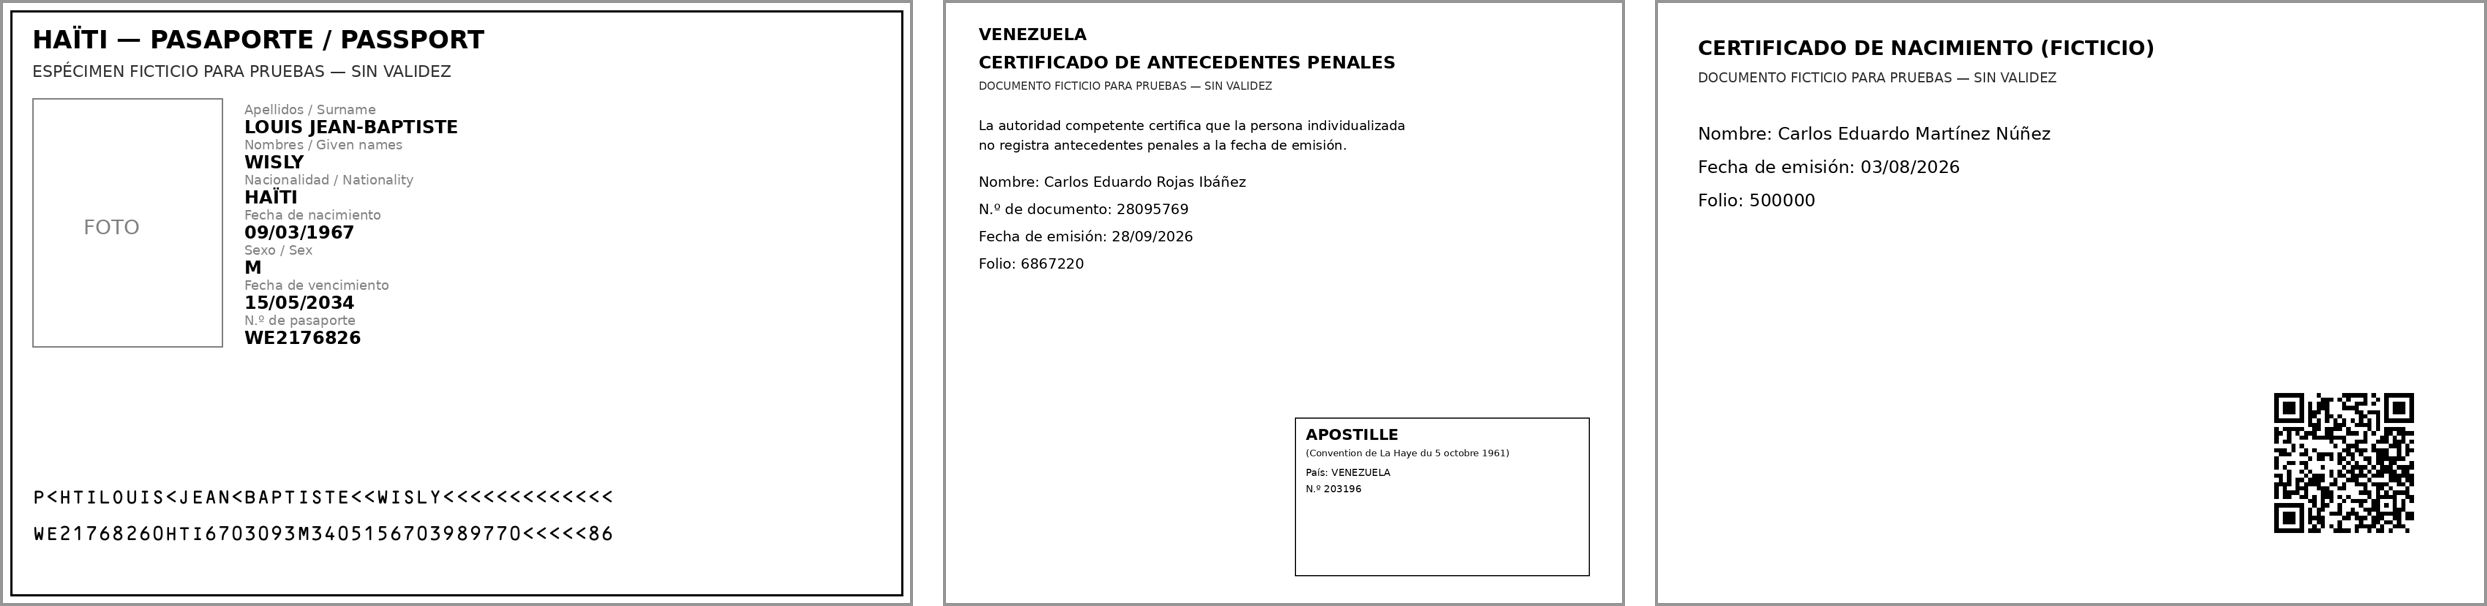
\includegraphics[width=\textwidth]{fig_maqueta_documentos.png}
\caption{Documentos ficticios generados por programa para probar la maqueta: pasaporte con la MRZ en tipografía OCR-B, certificado de antecedentes con apostilla y certificado chileno con código QR.}
\label{fig:docs}
\end{figure}

\begin{table}[!htbp]
\centering
\caption{Demostración: respuesta de la maqueta a documentos ficticios elegidos para recorrer cada vía. ``Derivado'' significa que el documento pasa a revisión humana sin imputarle un problema.}
\label{tab:demo}
\small
\begin{tabularx}{\textwidth}{L >{\raggedright\arraybackslash}p{2.7cm} >{\raggedright\arraybackslash}p{1.9cm} >{\raggedright\arraybackslash}p{4.3cm}}
\toprule
\textbf{Documento ficticio} & \textbf{Vía} & \textbf{Estado} & \textbf{Mensaje a la persona} \\
\midrule
Certificado chileno con código QR & Emisor & Prevalidado & --- \\
Certificado chileno con QR de otra persona & Emisor & Con alertas & El código de verificación corresponde a otra persona \\
Liquidación de sueldo con firma válida & Firma (texto del PDF firmado) & Prevalidado & --- \\
Liquidación con contenido agregado tras la firma & Firma y OCR & Con alertas & Se agregó contenido después de la firma \\
Pasaporte haitiano vigente & OCR de la MRZ & Prevalidado & --- \\
Pasaporte colombiano vencido & OCR de la MRZ & Con alertas & El pasaporte está vencido \\
Certificado de antecedentes venezolano con apostilla & OCR & Prevalidado & --- \\
Certificado de antecedentes haitiano sin legalización & OCR & Con alertas & No se detectó la legalización consular \\
Pasaporte boliviano con nombre levemente distinto del declarado & OCR de la MRZ & Derivado & El nombre del pasaporte difiere levemente del declarado: verificar \\
Certificado de antecedentes en criollo haitiano & Directo a revisión humana & Derivado & Idioma no soportado por el motor OCR \\
\bottomrule
\end{tabularx}
\end{table}

\subsubsection{Límites de la vía de firma}
\label{sec:limfirma}
La vía de firma de la maqueta se probó en condiciones favorables por construcción, y hay tres situaciones frecuentes en documentos reales que los corpus no contienen. Primero, la infraestructura simulada emite certificados con el RUT del empleador; si el documento lo firma una persona natural en nombre de la empresa, como su representante legal o un encargado de remuneraciones, el RUT del certificado no coincidirá con el de la empresa y la regla alertará sin fundamento. Mientras no se pueda verificar la representación, por ejemplo con registros de poderes, esa diferencia debería derivar y no alertar. Segundo, la maqueta valida solo la primera firma del PDF: en un contrato firmado por dos partes, la segunda firma se agrega después de la primera y el sistema la interpretaría como contenido agregado tras firmar, con una alerta injustificada; deben validarse todas las firmas y distinguir una firma posterior de otros cambios. Tercero, no se verifican la revocación del certificado ni el sello de tiempo.

\subsection{Problema metodológico detectado (PE3)}
\label{sec:metodologico}

Probar una maqueta construida por quien la diseña tiene un riesgo conocido: medirla con los mismos casos con que se ajustó. Este trabajo lo enfrentó en la práctica. La maqueta se construyó en cinco iteraciones y se probó con documentos ficticios generados por programa, y cada etapa mostró un aspecto distinto del mismo problema: lo que la maqueta parecía lograr dependía de cuánto se parecían los documentos de prueba a los de desarrollo. Esta subsección describe cómo se detectó; la siguiente propone cómo resolverlo. El detalle de las pruebas y sus cifras está en el Anexo~\ref{sec:anexo}.

\paragraph{Un corpus solo mide lo que contiene.} En las primeras iteraciones la maqueta parecía casi perfecta con los documentos de prueba. Una revisión del código encontró, sin embargo, defectos que esas pruebas no podían mostrar, porque los documentos no contenían los casos que los activaban: la validación de firma no detectaba contenido agregado después de firmar ni comparaba al firmante con el empleador, se exigía apostilla también a documentos haitianos, algunas reglas se evaluaban sobre lecturas no confiables y la bitácora no detectaba la eliminación de los últimos eventos. Se corrigieron, y se agregaron al generador documentos con esos casos (Anexo~\ref{sec:iteraciones}).

\paragraph{El artefacto de la tipografía de la MRZ.} Los primeros pasaportes ficticios imprimían la MRZ con una tipografía distinta de OCR-B, la que exige el Doc 9303 \cite{icao9303}, y el modelo genérico de Tesseract los leía casi sin errores. Al imprimirla en OCR-B, ese modelo validó poco más de la mitad de los pasaportes y leyó bien el nombre en muy pocos, porque confundía el carácter de relleno \texttt{<} con letras dentro del campo de nombres, que no está protegido por dígitos de control. Con un modelo entrenado para OCR-B \cite{doubango}, todos se leyeron correctamente (Anexo~\ref{sec:mrz}). La lectura casi perfecta inicial era, por tanto, un artefacto de documentos ficticios poco realistas. El hallazgo dejó además una consecuencia de diseño: un dígito de control válido no garantiza un nombre bien leído, por lo que una diferencia leve de nombre se deriva en vez de darse por buena.

\paragraph{Congelar el código y probar con documentos nuevos.} Para saber cómo se comportaba la maqueta ante documentos que no conocía, el código se congeló con una etiqueta en el repositorio y, \emph{después}, se escribió un segundo generador de documentos ficticios con condiciones ausentes del primero: diagramaciones y etiquetas nuevas, otros formatos de fecha y tipografías, tramas de fondo, timbres, fotocopias y fotografías degradadas. El resultado cambió la imagen de la maqueta (Anexo~\ref{sec:adversarial}). La propiedad central del diseño se sostuvo: ningún documento con un problema quedó dado por conforme en silencio, porque ante lo que no reconocía la maqueta derivaba. Pero derivó la mayoría de los documentos, sobre todo por condiciones que no conocía, y más de un tercio de sus alertas fue injustificado, por defectos de lógica que los documentos de desarrollo no activaban: la etiqueta francesa ``Nom'' coincidía con el comienzo de ``NOMBRE'' y la etiqueta ``Nombre'' con ``Nombre del padre'', de modo que se tomaba como nombre del titular un texto equivocado; un valor vacío se trataba como leído; y un RUT que no se pudo leer se trataba como distinto del firmante, en contra del principio de derivar ante la duda. Corregidos esos defectos, las alertas injustificadas casi desaparecieron con nuevos documentos del mismo generador, pero esa prueba ya no es independiente, porque las correcciones se hicieron viendo sus fallas.

\paragraph{La confianza del OCR no distinguió los errores.} El diseño inicial preveía derivar los campos leídos con baja confianza, con un umbral calibrado por idioma (sección~\ref{sec:umbral}). Con los documentos nuevos, subir el umbral redujo los campos aceptados sin mejorar su precisión: los errores se leían con confianza alta, porque provenían de tomar un texto equivocado, no de leer mal los caracteres (Anexo~\ref{sec:lectura}). Las derivaciones útiles vinieron de señales estructurales: una etiqueta no encontrada, una fecha que no se puede interpretar, un dígito de control que no cuadra. Por eso el principio 3 se reformuló como \emph{duda verificable} (sección~\ref{sec:principios}).

\paragraph{Medir por nacionalidad reveló un error sistemático.} Con una muestra mayor de certificados de antecedentes, la medición por nacionalidad mostró que el OCR leía el ordinal francés ``1er'' (primero) como ``ler'': la fecha no se podía interpretar y los certificados haitianos fechados el día 1 con ese ordinal se derivaban (Anexo~\ref{sec:muestra}). El error es seguro, porque deriva y no alerta, pero su costo recae en una nacionalidad, y solo se ve al medir por país con muestras suficientes.

\paragraph{Métricas precisadas después de ver resultados.} Algunas definiciones de las métricas se precisaron después de ver resultados: qué cuenta como un campo aceptado y cuándo una alerta acertó con la evidencia correcta y no por casualidad (Anexo~\ref{sec:metricas}). Las correcciones eran razonables, pero haberlas fijado antes habría evitado la duda de que se ajustaron a los resultados.

\paragraph{Los documentos de prueba contienen los problemas que las reglas buscan.} Los generadores introducen justamente los problemas que las reglas buscan, por lo que no prueban los modos de falla que nadie anticipó. Uno de ellos se identificó al revisar el código: el intérprete de fechas convierte ``1º de agosto'' en el 10 de agosto, porque normaliza la ``º'' como ``o'' y luego la corrige como un cero; un certificado emitido un día 1 que excediera la antigüedad máxima por menos de nueve días quedaría dado por conforme sin hallazgos. Además, la maqueta y los generadores se programaron con el mismo asistente de inteligencia artificial, lo que reduce la independencia de los documentos de prueba.

La Tabla~\ref{tab:lecciones} resume las observaciones, el problema metodológico que revela cada una y la solución que se propone en la subsección siguiente.

\begin{table}[!htbp]
\centering
\caption{Del problema observado a su solución.}
\label{tab:lecciones}
\small
\begin{tabularx}{\textwidth}{>{\raggedright\arraybackslash}p{4.2cm} >{\raggedright\arraybackslash}p{4.2cm} L}
\toprule
\textbf{Observación} & \textbf{Problema metodológico} & \textbf{Cómo resolverlo} \\
\midrule
Pruebas casi perfectas con documentos de desarrollo & El corpus solo contiene los casos previstos & Revisión del código y casos límite; corpus preparados por terceros \\
MRZ casi perfecta con una tipografía no estándar & Documentos ficticios poco realistas & Respetar los estándares (OCR-B) y usar conjuntos públicos como MIDV-2020 \\
Alertas injustificadas ante diagramaciones nuevas & Documentos de prueba parecidos a los de desarrollo & Congelar el código y evaluarlo una sola vez con documentos no vistos \\
La confianza del OCR no distinguió los errores & El umbral no puede calibrarse con documentos sintéticos & Señales estructurales de duda; calibración con documentos reales \\
Error del ordinal francés concentrado en certificados haitianos & Muestras pequeñas por nacionalidad & Medir por nacionalidad con muestras planificadas \\
Métricas precisadas después de ver resultados & Riesgo de ajustar la medición a los resultados & Fijar métricas y criterios antes de evaluar \\
Omisión posible con fechas como ``1º de agosto'' & Los corpus contienen solo los problemas que las reglas buscan & Incluir modos realistas de falla y documentos reales \\
Maqueta y generadores del mismo origen & Falta de independencia & Corpus de terceros y documentos reales anonimizados \\
\bottomrule
\end{tabularx}
\end{table}

\subsection{Protocolo de evaluación propuesto (PE3)}
\label{sec:pendiente}

Los problemas de la subsección anterior no se resuelven con más pruebas del mismo tipo, sino con un protocolo que separe a quien construye de quien evalúa y fije de antemano qué se medirá. El protocolo propuesto sigue la estrategia de FEDS \cite{venable2016} y tiene cuatro componentes.

\subsubsection{Criterios fijados antes de evaluar}
Antes de cada evaluación se registran, con fecha, las métricas y los criterios de aceptación, derivados de los requerimientos:
\begin{itemize}
  \item \textbf{Seguridad}: ningún documento con un problema queda prevalidado (omisión silenciosa). Si no hay omisiones, se informa la cota superior unilateral al 95\,\% sobre los documentos con problemas.
  \item \textbf{Eficacia}: la precisión estricta de lo aceptado debe cumplir RNF-04 en cada idioma, lo que exige al menos 299 campos aceptados por idioma (sección~\ref{sec:umbral}), y las alertas injustificadas deben cumplir RNF-06 en cada idioma.
  \item \textbf{Equidad}: la derivación y las alertas injustificadas no difieren significativamente entre nacionalidades (prueba de independencia, $\alpha$ = 0,05), con muestras dimensionadas para detectar diferencias relevantes; los tiempos de resolución por nacionalidad se miden en el piloto (RNF-07).
  \item \textbf{Cobertura}: la derivación debe quedar bajo la derivación máxima con que el sistema ahorra horas (sección~\ref{sec:impacto}).
\end{itemize}
Las métricas se informan por idioma y nacionalidad: detección de problemas con la evidencia correcta, omisiones silenciosas y con derivación, documentos con alertas injustificadas, proporción de alertas injustificadas, derivación y precisión de lectura en versión estricta.

\subsubsection{Secuencia y corpus de evaluación}
\begin{enumerate}
  \item \textbf{Desarrollo} con un corpus propio, que solo sirve para construir.
  \item \textbf{Congelamiento} del código con una etiqueta en el repositorio.
  \item \textbf{Evaluación única} con documentos que el equipo de desarrollo no conoce: documentos ficticios preparados por terceros, conjuntos públicos como MIDV-2020 \cite{bulatov2022} para la lectura de la MRZ y, con autorización del Servicio, documentos reales anonimizados. Los corpus deben incluir modos realistas de falla (documentos con varias fechas, parientes con nombres compartidos, fechas con ordinales como ``1º'') y una prevalencia de problemas similar a la de los expedientes reales.
  \item \textbf{Corrección} de los defectos y nueva evaluación con un corpus nuevo, nunca con el mismo.
  \item \textbf{Comparación de motores}: ejecutar los mismos corpus con Textract, Azure y Document AI mediante los adaptadores implementados, con una muestra de calibración de al menos 300 campos por idioma.
\end{enumerate}

\subsubsection{Modelo de impacto}
\label{sec:impacto}
Esta subsección presenta escenarios con supuestos explícitos, no resultados medidos. La Tabla~\ref{tab:costos} (Anexo~\ref{sec:anexob}) estima el costo operativo del OCR en la nube: entre USD 47.725 y 115.225 anuales según el número de páginas por solicitud, de 0,32 a 0,77 dólares por solicitud; y la Tabla~\ref{tab:sensibilidad}, las horas que podría liberar.

Con el precio de formularios de Google Document AI (USD 0,03 por página \cite{googlepricing}) y el mismo precio por la página del pasaporte, el escenario de 6 páginas bajaría a unos USD 22.725 anuales en OCR. Con Tesseract no hay costo por página, pero sí de infraestructura y operación propias. Los USD 10.000 de infraestructura son una estimación de orden de magnitud. El escenario es conservador: supone que todas las páginas pasan por OCR, mientras que en el diseño híbrido las que se verifican con el emisor o por firma no lo requieren. El costo de implementación y el ahorro monetario no se cuantifican.

\paragraph{Horas de trabajo liberadas.}
Por diseño, un documento derivado vuelve a la revisión completa, por lo que solo los documentos no derivados pueden ahorrar tiempo; el modelo supone, además, que derivar no agrega tiempo a la revisión actual. El ahorro neto de horas se expresa a partir de los tiempos por documento:
\[
H_{\mathrm{neto}} = M \left[ (1-d)\, t_{a} - a \, p_{f} \, t_{f} \right],
\]
donde $M$ es el número de documentos procesados al año, $d$ la proporción de documentos derivados, $t_{a}$ el tiempo ahorrado en cada documento no derivado, $a$ el número medio de alertas por documento, $p_{f}$ la proporción de alertas injustificadas y $t_{f}$ el tiempo que cuesta descartar una alerta injustificada, con los tiempos expresados en horas. La evaluación técnica del protocolo estimará $d$, $a$ y $p_f$; $t_a$ y $t_f$ deben medirse con funcionarios.

La Tabla~\ref{tab:sensibilidad} muestra el primer término para 150.000 solicitudes con cuatro documentos procesados por solicitud (pasaporte, certificado de antecedentes y dos documentos privados), es decir, 600.000 documentos al año. Con $d = 0$, los escenarios coinciden con 2, 6 y 10 minutos ahorrados por solicitud. En el escenario intermedio (1,5 minutos por documento) con una derivación del 30\,\%, el ahorro bruto sería de 10.500 horas anuales, cerca de 5,2 funcionarios a jornada completa, considerando la jornada de 44 horas semanales del Estatuto Administrativo \cite{estatuto} y 46 semanas efectivas (2.024 horas anuales).

\begin{table}[!htbp]
\centering
\caption{Horas anuales ahorradas antes de descontar las alertas injustificadas, $M (1-d)\, t_a$ (con $t_a$ convertido a horas), para 600.000 documentos al año.}
\label{tab:sensibilidad}
\small
\begin{tabular}{lrrr}
\toprule
\textbf{Derivación $d$} & \textbf{$t_a$ = 0,5 min} & \textbf{$t_a$ = 1,5 min} & \textbf{$t_a$ = 2,5 min} \\
\midrule
0\,\% (referencia) & 5.000 & 15.000 & 25.000 \\
15\,\% & 4.250 & 12.750 & 21.250 \\
30\,\% & 3.500 & 10.500 & 17.500 \\
50\,\% & 2.500 & 7.500 & 12.500 \\
\bottomrule
\end{tabular}
\end{table}

El segundo término muestra por qué importan las alertas injustificadas. Igualando ambos términos se obtiene la derivación máxima con la que el sistema todavía ahorra horas: $d^{*} = 1 - a\,p_f\,t_f / t_a$. Por ejemplo, con media alerta por documento ($a$ = 0,5), $t_a$ = 1,5 y $t_f$ = 5 minutos, si el 5\,\% de las alertas es injustificado, el sistema ahorra horas mientras derive menos del 92\,\% de los documentos; si lo es un 35\,\%, cerca de lo observado con la maqueta ante diagramaciones nuevas, el límite baja a cerca del 42\,\%. A ese costo se suma el de las personas solicitantes que reemplazan sin necesidad un documento válido, que el modelo no incluye. Tampoco incluye el beneficio que motiva el diseño, la reducción de requerimientos de antecedentes y de su plazo de hasta 60 días, porque no hay datos públicos sobre su frecuencia (sección~\ref{sec:diagnostico}).

\subsubsection{Evaluación naturalista}
La evaluación naturalista requiere acceso a personas y datos que exceden el alcance de este trabajo y queda definida así:
\begin{itemize}
  \item \textbf{Estudio de tiempos}: medir con funcionarios o evaluadores la revisión de expedientes ficticios con y sin prevalidación para estimar $t_a$ y $t_f$, y la frecuencia con que corrigen o descartan alertas.
  \item \textbf{Juicio de expertos}: entre tres y cinco expertos (funcionarios o exfuncionarios de migraciones, abogados migratorios y especialistas en gobierno digital) evalúan el diseño y las reglas; se reportan el índice de validez de contenido, el acuerdo entre evaluadores y las modificaciones incorporadas.
  \item \textbf{Solicitud de información}: mediante la Ley N.º 20.285 \cite{ley20285}, solicitar al SERMIG el número de solicitudes pendientes, los requerimientos de antecedentes emitidos y sus causas, y los tiempos por etapa.
  \item \textbf{Piloto}: de 2 a 3 meses, en paralelo con el proceso manual, con documentos reales y los criterios RNF-04, RNF-06 y RNF-07, que permita además calibrar el umbral de confianza.
\end{itemize}

\paragraph{Síntesis de PE3.} La maqueta demuestra que el diseño es implementable con tecnologías de código abierto: recorre las tres vías de verificación, aplica las reglas, deriva lo dudoso y registra cada evento. Probarla mostró el problema metodológico central de este tipo de sistemas: con documentos ficticios parecidos a los de desarrollo, la maqueta parece mejor de lo que es. La respuesta es un protocolo que fija los criterios antes de evaluar, evalúa una sola vez el código congelado con documentos que el equipo no conoce, mide por nacionalidad y termina con funcionarios y documentos reales.

% ---------------------------------------------------------------------
\section{Discusión}
\label{sec:discusion}

Lo observado al probar la maqueta dialoga con la literatura en cinco puntos y deja, además, una lectura propia de la ciencia del diseño.

\paragraph{Lectura de pasaportes.} Liu et al. reportan una detección de la MRZ del 100\,\% y un F1 de reconocimiento de caracteres de 98,36\,\% con redes convolucionales \cite{liu2021}. En la última iteración de la maqueta, con Tesseract y un modelo para OCR-B, la MRZ se leyó de forma confiable en imágenes limpias, pero no en fotografías de celular con fuerte degradación. Las observaciones no son comparables, porque los documentos de este trabajo son ficticios, pero indican que la lectura de pasaportes fotografiados por las propias personas, el caso típico de un portal, requiere un motor más robusto o un control de calidad de la imagen al cargarla (RF-02).

\paragraph{Motores y degradación.} Hegghammer encontró que los servicios en la nube superan ampliamente a Tesseract en imágenes con ruido \cite{hegghammer2022}. En las pruebas de la maqueta con documentos nuevos, la derivación fue mucho mayor en fotografías de celular con fuerte degradación que en imágenes limpias (Anexo~\ref{sec:degradacion}), por lo que la comparación de motores es la parte del protocolo con más potencial para reducirlas.

\paragraph{Diagramaciones.} Cutting y Cutting-Decelle identifican los documentos poco estructurados como el principal desafío práctico \cite{cutting2021}, y las pruebas lo confirman: las alertas injustificadas del código congelado vinieron sobre todo de diagramaciones y etiquetas nuevas, más que de errores de caracteres. Los modelos que combinan texto, imagen y posición \cite{huang2022} son la alternativa natural a la extracción por etiquetas, siempre que entreguen una señal de duda útil.

\paragraph{Opción de rechazo.} En la teoría de la opción de rechazo, la abstención se decide con una confianza calibrada \cite{chow1970,geifman2017}. En la maqueta, la confianza del OCR distinguió mal los errores, y las abstenciones útiles vinieron de señales estructurales. En documentos, la duda parece detectarse mejor con controles de consistencia que con la confianza del reconocedor, lo que acerca el diseño a la verificación cruzada entre campos y documentos.

\paragraph{Sesgo de automatización y equidad.} Las pruebas dan contenido al riesgo de sesgo de automatización \cite{parasuraman2010,alonbarkat2023}: ante diagramaciones nuevas, más de un tercio de las alertas de la maqueta fue injustificado. Si los funcionarios confiaran en ellas, el sistema produciría errores en vez de evitarlos; si aprendieran a ignorarlas, perdería su valor. El error del ordinal francés muestra, en pequeño, el riesgo que motiva el principio 3: un detalle de formato de un idioma concentró derivaciones en una nacionalidad, y solo se vio al medir por país con una muestra suficiente.

\paragraph{Lo aprendido como conocimiento de diseño.} En ciencia del diseño, una evaluación que muestra dónde falla un artefacto también produce conocimiento de diseño \cite{hevner2004,venable2016}. El problema metodológico observado no invalida los principios, pero los precisa: la seguridad del diseño se apoya en derivar ante señales estructurales, no en la confianza del reconocedor, y su eficacia depende de extraer los datos ante diagramaciones variadas. Ambas conclusiones orientan el protocolo propuesto.

\subsection{Escalabilidad}

La lógica del sistema puede extenderse a otros trámites con revisión documental, como la residencia temporal o la nacionalización, incorporando reglas en la configuración. A medida que más emisores ofrezcan verificación electrónica, más documentos pasarán de la vía OCR a la del emisor, en línea con la Ley N.º 21.180 \cite{ley21180}. Las pruebas de la maqueta apuntan en esa dirección, porque la lectura por OCR fue la principal fuente de derivaciones, aunque la vía de firma se evaluó en condiciones favorables (sección~\ref{sec:limfirma}). Los principios de diseño podrían servir a otros organismos que gestionan documentación ciudadana heterogénea, cuya validación con documentos reales forma parte del protocolo propuesto (sección~\ref{sec:pendiente}).

\subsection{Implicancias éticas}
\label{sec:etica}

\paragraph{Equidad y discriminación indirecta.} Las pruebas de la maqueta ilustraron el riesgo que motiva el principio 3: un error de lectura del ordinal francés concentró derivaciones en certificados haitianos (sección~\ref{sec:metodologico}), y en las primeras iteraciones un error sistemático en la MRZ había afectado a pasaportes haitianos. El diseño evita que esos errores se traduzcan en alertas injustificadas, pero los desplaza a la revisión humana, lo que puede alargar el trámite de quienes presentan documentos más difíciles de leer. Aunque las derivaciones no son decisiones automatizadas en el sentido del artículo 8 bis de la Ley N.º 19.628 (sección~\ref{sec:cumplimiento}), una demora sistemáticamente mayor para una nacionalidad podría constituir discriminación indirecta, por lo que RNF-07 exige medir en el piloto los tiempos de resolución por nacionalidad, y la evaluación de impacto en protección de datos debe considerarlo.

\paragraph{Revisión humana y proporcionalidad.} El sistema puede advertir, pero nunca rechazar. En el caso resuelto por la Corte Suprema \cite{cs2026}, la mayoría validó el rechazo de una solicitud por un certificado adulterado, mientras el voto disidente lo consideró desproporcionado atendida la imposibilidad alegada de obtener el documento. Situaciones como esta requieren ponderación humana.

\paragraph{Accesibilidad y gobernanza de los datos.} La plataforma debe cumplir WCAG 2.2 nivel AA \cite{wcag22}, ofrecer una interfaz multilingüe y mantener atención presencial. Los documentos contienen datos de especial protección, como antecedentes penales, cuyo tratamiento debe cumplir con minimización, transparencia sobre las reglas aplicadas y auditoría, bajo la supervisión del Servicio, la Agencia de Protección de Datos Personales y el Consejo para la Transparencia.

% ---------------------------------------------------------------------
\section{Conclusiones}

Este trabajo se preguntó cómo diseñar un sistema de prevalidación documental para la residencia definitiva que reduzca la carga de revisión del Servicio Nacional de Migraciones sin automatizar decisiones ni dar por conforme en silencio un documento con problemas. La respuesta se construye a partir de las tres preguntas específicas.

\paragraph{PE1: el problema.} La revisión documental se concentra en la revisión formal al acoger la solicitud, que termina en requerimientos con hasta 60 días de plazo, y en la revisión de fondo. Los documentos exigidos se dividen por su origen en públicos chilenos, privados con firma electrónica y extranjeros o privados sin firma, y cada grupo admite, en general, una vía de verificación distinta. El OCR, por tanto, no reemplaza a la interoperabilidad: cubre lo que esta no alcanza.

\paragraph{PE2: la arquitectura.} La solución verifica cada documento por la vía más confiable disponible ---emisor, firma u OCR---, con reglas configurables que solo alertan o derivan y una regla transversal: ante la duda, derivar. La arquitectura mantiene los datos en Chile y hace intercambiable el motor OCR, y la contrastación normativa muestra que el diseño es compatible con el marco chileno, siempre que se mida cómo usan los funcionarios las alertas. El conocimiento de diseño se resume en tres principios: primero el emisor, con el OCR como respaldo; advertir, nunca rechazar, y ante la duda derivar; y duda verificable con equidad medida.

\paragraph{PE3: la maqueta y el problema metodológico.} La maqueta funcional demuestra que el diseño es implementable con tecnologías de código abierto: recorre las tres vías, aplica las reglas, deriva lo dudoso y registra cada evento. Probarla reveló el problema metodológico central de este tipo de sistemas: con documentos ficticios parecidos a los de desarrollo, la maqueta parecía casi perfecta, y esa imagen no se sostuvo ante documentos con diagramaciones nuevas generados después de congelar el código. En esos casos el diseño falló de manera segura ---derivó lo que no conocía en vez de darlo por conforme---, pero con muchas derivaciones y alertas injustificadas. La solución propuesta es un protocolo que fija los criterios antes de evaluar, evalúa una sola vez el código congelado con documentos que el equipo no conoce, mide por nacionalidad y termina con un estudio de tiempos, un juicio de expertos y un piloto con documentos reales.

\paragraph{Respuesta a la pregunta general.} El sistema puede diseñarse combinando las tres vías bajo el principio de derivar ante la duda, y la maqueta muestra que ese diseño es técnicamente realizable. Si reduce la carga de revisión depende de cuántos documentos reales logre leer con confianza y del tiempo que ahorre a los funcionarios, lo que el protocolo propuesto permitirá medir. El aporte del trabajo no es una cifra de precisión, sino un diseño cuyas fallas, en los casos probados, no dieron por conforme ningún documento con problemas y quedaron a la vista, y una forma de evaluarlo que evita el optimismo de los documentos sintéticos.

El problema que motiva el trabajo sigue vigente: la residencia definitiva registró 133.726 otorgamientos en 2024 \cite{sermig2025}, y su único dato público de duración, para niños, niñas y adolescentes, promedió 770 días entre 2022 y 2024 \cite{defensoria2026}, muy por encima del plazo de seis meses de la Ley N.º 19.880 \cite{ley19880}.

\paragraph{Aportes.} El trabajo aporta un artefacto de diseño para la prevalidación documental migratoria (flujos, requerimientos, reglas y una arquitectura independiente del proveedor), una maqueta funcional de código abierto que lo implementa, tres principios de diseño y un protocolo de evaluación que responde a un problema metodológico documentado en la práctica.

\subsection{Limitaciones}
La maqueta se probó solo con documentos ficticios y con un motor OCR, Tesseract, sin calibrar el umbral de confianza; el emisor y la infraestructura de firma son simulados, y la vía de firma se probó en condiciones favorables (sección~\ref{sec:limfirma}). Los documentos de prueba y la maqueta se programaron con el mismo asistente de inteligencia artificial, y algunas métricas se precisaron después de ver resultados. La maqueta conserva defectos conocidos, entre ellos un modo de omisión silenciosa con fechas como ``1º de agosto''. El diagnóstico se basa en fuentes públicas, sin observación directa del proceso interno ni datos del número de solicitudes pendientes. El tiempo ahorrado y la carga de las alertas sobre los funcionarios no se midieron. La revisión de literatura no fue sistemática.

\subsection{Trabajo futuro}
\begin{itemize}
  \item Ejecutar el protocolo de evaluación (sección~\ref{sec:pendiente}), en particular el estudio de tiempos, el juicio de expertos y la prueba con documentos reales y motores en la nube.
  \item Implementar el portal del solicitante y el panel del funcionario, con la corrección de datos (RF-11), y evaluar su usabilidad.
  \item Ajustar la regla del firmante para documentos firmados por representantes, validar todas las firmas del PDF y verificar la revocación y el sello de tiempo.
  \item Corregir los defectos conocidos de la maqueta (el intérprete de fechas con ordinales como ``1º'' y ``1er'', la detección de la apostilla ante errores de espaciado del OCR, la comparación de nombres truncados cuando el nombre declarado omite un segundo nombre y la de nombres con palabras unidas) y reevaluarla con un corpus nuevo.
  \item Reducir la derivación sin sacrificar la seguridad: extracción por posición y no solo por etiqueta, y modelos de diagramación como LayoutLMv3 o modelos multimodales mediante el adaptador.
  \item Buscar señales de duda distintas de la confianza del OCR, como la consistencia entre campos y documentos o el acuerdo entre dos motores, y calibrarlas con documentos reales.
  \item Verificar la autenticidad de documentos extranjeros mediante interoperabilidad con autoridades emisoras.
  \item Realizar una revisión sistemática de la literatura sobre prevalidación documental en el sector público.
\end{itemize}

\paragraph{Disponibilidad del código.} El código de la maqueta, los generadores de documentos ficticios, los scripts de prueba y de figuras y los archivos de resultados acompañan este trabajo en un repositorio git, con etiquetas para la iteración 3, el código congelado y la iteración 5. Las cifras del Anexo~\ref{sec:anexo}, en particular las de las Tablas~\ref{tab:resultados}, \ref{tab:deteccion}, \ref{tab:condiciones} y \ref{tab:lineabase} y de las Figuras~\ref{fig:evaluaciones} y \ref{fig:pais}, provienen de los archivos de métricas de cada evaluación mediante los scripts \texttt{razon\_correcta.py} y \texttt{figuras.py}. Los corpus pueden regenerarse con los generadores y las semillas de la Tabla~\ref{tab:corpus}. Las iteraciones 1 y 2 no se versionaron por separado.

\paragraph{Declaración de uso de inteligencia artificial.} El tema, el planteamiento del problema y la versión inicial de este trabajo son de la autora. El código de la maqueta, los generadores de documentos ficticios, la ejecución de las pruebas y buena parte de la redacción de esta versión se realizaron con un asistente de inteligencia artificial generativa (Claude, de Anthropic) en octubre de 2026, a partir de las indicaciones y revisiones de la autora. Las revisiones críticas de cada versión también se hicieron con ese asistente, no con evaluadores humanos. Entre las decisiones de la autora están el tema y el alcance, el enfoque del trabajo en la arquitectura, la maqueta y el problema metodológico, la estructura del documento, la exclusión de estimaciones monetarias del ahorro y la decisión de someter cada versión a esas revisiones críticas. El historial del repositorio refleja ese proceso. La autora es responsable del contenido, de la verificación de las fuentes y de los resultados reportados.

% ---------------------------------------------------------------------
\begin{thebibliography}{99}
\small
\bibitem{alonbarkat2023}
Alon-Barkat, S., \& Busuioc, M. (2023). Human--AI interactions in public sector decision making: ``Automation bias'' and ``selective adherence'' to algorithmic advice. \emph{Journal of Public Administration Research and Theory, 33}(1), 153--169. \url{https://doi.org/10.1093/jopart/muac007}

\bibitem{awschile}
Amazon Web Services. (2025). \emph{Coming soon: AWS South America (Chile) Region}. AWS News Blog. \url{https://aws.amazon.com/blogs/aws/coming-soon-aws-south-america-chile-region/}

\bibitem{awsoptout}
Amazon Web Services. (2026). \emph{AI services opt-out policies}. AWS Organizations User Guide. \url{https://docs.aws.amazon.com/organizations/latest/userguide/orgs_manage_policies_ai-opt-out.html}

\bibitem{awsendpoints}
Amazon Web Services. (2026). \emph{Amazon Textract endpoints and quotas}. AWS General Reference. \url{https://docs.aws.amazon.com/general/latest/gr/textract.html}

\bibitem{awsfaq}
Amazon Web Services. (2026). \emph{Amazon Textract FAQs}. \url{https://aws.amazon.com/textract/faqs/}

\bibitem{awspricing}
Amazon Web Services. (2026). \emph{Amazon Textract pricing}. \url{https://aws.amazon.com/textract/pricing/}

\bibitem{awsid}
Amazon Web Services. (2026). \emph{Analyzing identity documents}. Amazon Textract Developer Guide. \url{https://docs.aws.amazon.com/textract/latest/dg/how-it-works-identity.html}

\bibitem{bansak2018}
Bansak, K., Ferwerda, J., Hainmueller, J., Dillon, A., Hangartner, D., Lawrence, D., \& Weinstein, J. (2018). Improving refugee integration through data-driven algorithmic assignment. \emph{Science, 359}(6373), 325--329. \url{https://doi.org/10.1126/science.aao4408}

\bibitem{bcn21719}
Biblioteca del Congreso Nacional de Chile. (2024). \emph{Balance legislativo de la Ley 21.719}. \url{https://www.bcn.cl/balance-legislativo/detalle/ficha_LEY_21719_2024-12-13}

\bibitem{bulatov2022}
Bulatov, K., Emelianova, E., Tropin, D., Skoryukina, N., Chernyshova, Y., Sheshkus, A., Usilin, S., Ming, Z., Burie, J.-C., Luqman, M. M., \& Arlazarov, V. V. (2022). MIDV-2020: A comprehensive benchmark dataset for identity document analysis. \emph{Computer Optics, 46}(2). \url{https://computeroptics.ru/KO/Annot/KO46-2/460212.html}

\bibitem{busuioc2021}
Busuioc, M. (2021). Accountable artificial intelligence: Holding algorithms to account. \emph{Public Administration Review, 81}(5), 825--836. \url{https://doi.org/10.1111/puar.13293}

\bibitem{cariola2026}
Cariola Díez Pérez-Cotapos. (2026, 2 de septiembre). \emph{Alerta legal: Proyecto de ley que prorroga la entrada en vigencia de la Ley N.º 21.719}. \url{https://www.cariola.cl/app/uploads/2026/09/Alerta-legal_-2septiembre.pdf}

\bibitem{chow1970}
Chow, C. K. (1970). On optimum recognition error and reject tradeoff. \emph{IEEE Transactions on Information Theory, 16}(1), 41--46. \url{https://doi.org/10.1109/TIT.1970.1054406}

\bibitem{clopper1934}
Clopper, C. J., \& Pearson, E. S. (1934). The use of confidence or fiducial limits illustrated in the case of the binomial. \emph{Biometrika, 26}(4), 404--413. \url{https://doi.org/10.1093/biomet/26.4.404}

\bibitem{hcch2026}
Conferencia de La Haya de Derecho Internacional Privado (HCCH). (2026). \emph{Status table: Convention of 5 October 1961 Abolishing the Requirement of Legalisation for Foreign Public Documents} (actualizada al 30 de junio de 2026). \url{https://www.hcch.net/en/instruments/conventions/status-table/?cid=41}

\bibitem{cs2026}
Corte Suprema de Chile. (2026). \emph{Sentencia Rol N.º 6.236-2025}. Texto publicado por Diario Constitucional. \url{https://www.diarioconstitucional.cl/2026/01/25/corte-suprema-revoca-fallo-y-valida-rechazo-de-residencia-definitiva-por-certificado-de-antecedentes-adulterado/}

\bibitem{cui2021}
Cui, L., Xu, Y., Lv, T., \& Wei, F. (2021). \emph{Document AI: Benchmarks, models and applications} (preprint). arXiv:2111.08609. \url{https://arxiv.org/abs/2111.08609}

\bibitem{cutting2021}
Cutting, G. A., \& Cutting-Decelle, A.-F. (2021). \emph{Intelligent document processing: Methods and tools in the real world} (preprint). arXiv:2112.14070. \url{https://arxiv.org/abs/2112.14070}

\bibitem{dasd2026}
Das, D., Tamura, M., Ahmed, S. I., \& Guha, S. (2026). ``Is this not enough?'': Asymmetries in institutional accountability and collective sensemaking in the case of Canada's algorithmic visa triage system. En \emph{ACM SIGCAS/SIGCHI Conference on Computing and Sustainable Societies (COMPASS '26)}. \url{https://doi.org/10.1145/3811242.3819106}

\bibitem{das2026}
Das, G., Kumar C, P., \& Ramachandra, R. (2026). \emph{From forgeries to foundation models: A systematic survey of identity document attack and detection} (preprint). arXiv:2607.01442. \url{https://arxiv.org/abs/2607.01442}

\bibitem{mschile}
DatacenterDynamics. (2025, 19 de junio). \emph{Microsoft launches Chile cloud region}. \url{https://www.datacenterdynamics.com/en/news/microsoft-launches-chile-cloud-region/}

\bibitem{estatuto}
Decreto con Fuerza de Ley N.º 29 que fija el texto refundido, coordinado y sistematizado de la Ley N.º 18.834 sobre Estatuto Administrativo, art. 65. (2005). \url{https://www.bcn.cl/leychile/navegar?idNorma=236392}

\bibitem{decreto177}
Decreto N.º 177 que establece las subcategorías migratorias de residencia temporal. (2022). Ministerio del Interior y Seguridad Pública. \url{https://www.bcn.cl/leychile/navegar?idNorma=1176043}

\bibitem{defensoria2026}
Defensoría de la Niñez. (2026). \emph{Documento de trabajo N.º 10: Duración de procesos administrativos de migración de niños, niñas y adolescentes}. \url{https://observatorio.defensorianinez.cl/wp-content/uploads/2026/02/Documento-de-trabajo-10-Duracion-de-procesos-administrativos-de-migracion-de-ninos-ninas-y-adolescentes.pdf}

\bibitem{doubango}
DoubangoTelecom. (2019). \emph{tesseractMRZ: Tesseract model for machine-readable zones} (licencia BSD-3). GitHub. \url{https://github.com/DoubangoTelecom/tesseractMRZ}

\bibitem{engstrom2020}
Engstrom, D. F., Ho, D. E., Sharkey, C. M., \& Cuéllar, M.-F. (2020). \emph{Government by algorithm: Artificial intelligence in federal administrative agencies}. Informe para la Administrative Conference of the United States. \url{https://www.law.stanford.edu/wp-content/uploads/2020/02/ACUS-AI-Report.pdf}

\bibitem{geifman2017}
Geifman, Y., \& El-Yaniv, R. (2017). Selective classification for deep neural networks. En \emph{Advances in Neural Information Processing Systems 30 (NeurIPS 2017)} (pp. 4878--4887). \url{https://arxiv.org/abs/1705.08500}

\bibitem{latercera2023}
González, E. (2023, 26 de noviembre). El pujante y cuestionado negocio de los abogados migratorios. \emph{La Tercera}.

\bibitem{googleid}
Google Cloud. (2022, 1 de junio). \emph{Google Cloud extends Document AI with new parsers for identity}. Google Cloud Blog. \url{https://cloud.google.com/blog/products/ai-machine-learning/google-cloud-extends-document-ai-with-new-parsers-for-identity/}

\bibitem{googlepricing}
Google Cloud. (2026). \emph{Document AI pricing}. \url{https://cloud.google.com/document-ai/pricing}

\bibitem{gdocairegions}
Google Cloud. (2026). \emph{Document AI: Regional and multi-regional support}. \url{https://cloud.google.com/document-ai/docs/regions}

\bibitem{ircc2022}
Government of Canada, Immigration, Refugees and Citizenship Canada. (2022). \emph{Advanced data analytics to sort and help process temporary resident visa applications}. \url{https://www.canada.ca/en/immigration-refugees-citizenship/corporate/transparency/committees/cimm-feb-15-17-2022/advanced-data-analytics-sort-process-trv.html}

\bibitem{canada2019}
Government of Canada, Treasury Board Secretariat. (2019). \emph{Directive on Automated Decision-Making}. \url{https://www.tbs-sct.canada.ca/pol/doc-eng.aspx?id=32592}

\bibitem{gregor2013}
Gregor, S., \& Hevner, A. R. (2013). Positioning and presenting design science research for maximum impact. \emph{MIS Quarterly, 37}(2), 337--355. \url{https://doi.org/10.25300/MISQ/2013/37.2.01}

\bibitem{gregor2020}
Gregor, S., Kruse, L. C., \& Seidel, S. (2020). Research perspectives: The anatomy of a design principle. \emph{Journal of the Association for Information Systems, 21}(6), 1622--1652. \url{https://doi.org/10.17705/1jais.00649}

\bibitem{hegghammer2022}
Hegghammer, T. (2022). OCR with Tesseract, Amazon Textract, and Google Document AI: a benchmarking experiment. \emph{Journal of Computational Social Science, 5}(1), 861--882. \url{https://doi.org/10.1007/s42001-021-00149-1}

\bibitem{hevner2004}
Hevner, A. R., March, S. T., Park, J., \& Ram, S. (2004). Design science in information systems research. \emph{MIS Quarterly, 28}(1), 75--105. \url{https://doi.org/10.2307/25148625}

\bibitem{huang2022}
Huang, Y., Lv, T., Cui, L., Lu, Y., \& Wei, F. (2022). LayoutLMv3: Pre-training for document AI with unified text and image masking. En \emph{Proceedings of the 30th ACM International Conference on Multimedia} (pp. 4083--4091). \url{https://doi.org/10.1145/3503161.3548112}

\bibitem{ine2024}
Instituto Nacional de Estadísticas y Servicio Nacional de Migraciones. (2024, 30 de diciembre). \emph{Estimación de personas extranjeras residentes habituales en Chile 2023}. \url{https://serviciomigraciones.cl/sermig-e-ine-presentaron-estimacion-de-personas-extranjeras-residentes-habituales-en-chile-2023/}

\bibitem{icao9303}
International Civil Aviation Organization. (2021). \emph{Doc 9303: Machine Readable Travel Documents} (8.ª ed.). \url{https://www.icao.int/publications/pages/publication.aspx?docnum=9303}

\bibitem{iso32000}
International Organization for Standardization. (2020). \emph{ISO 32000-2:2020 Document management --- Portable document format --- Part 2: PDF 2.0}.

\bibitem{iso27001}
International Organization for Standardization. (2022). \emph{ISO/IEC 27001:2022 Information security, cybersecurity and privacy protection --- Information security management systems --- Requirements}.

\bibitem{jdf2026}
Jara, S. (2026, 19 de octubre). \emph{Comisión de Constitución aprueba en general la postergación de la entrada en vigencia de la Ley N.º 21.719 sobre Protección de Datos Personales}. JDF Jara del Favero. \url{https://jdf.cl/en/comision-de-constitucion-aprueba-en-general-la-postergacion-de-la-entrada-en-vigencia-de-la-ley-n21-719-sobre-proteccion-de-datos-personales/}

\bibitem{krimmer2017}
Krimmer, R., Kalvet, T., Toots, M., Cepilovs, A., \& Tambouris, E. (2017). Exploring and demonstrating the once-only principle: A European perspective. En \emph{Proceedings of the 18th Annual International Conference on Digital Government Research (dg.o 2017)} (pp. 546--551). ACM. \url{https://doi.org/10.1145/3085228.3085235}

\bibitem{toop2021}
Krimmer, R., Prentza, A., \& Mamrot, S. (Eds.). (2021). \emph{The once-only principle: The TOOP project} (Lecture Notes in Computer Science, vol. 12621). Springer. \url{https://doi.org/10.1007/978-3-030-79851-2}

\bibitem{levenshtein1966}
Levenshtein, V. I. (1966). Binary codes capable of correcting deletions, insertions, and reversals. \emph{Soviet Physics Doklady, 10}(8), 707--710.

\bibitem{ley19628}
Ley N.º 19.628 sobre Protección de la Vida Privada. (1999). \url{https://www.bcn.cl/leychile/navegar?idNorma=141599}

\bibitem{ley19799}
Ley N.º 19.799 sobre documentos electrónicos, firma electrónica y servicios de certificación de dicha firma. (2002). \url{https://www.bcn.cl/leychile/navegar?idNorma=196640}

\bibitem{ley19880}
Ley N.º 19.880 que establece bases de los procedimientos administrativos que rigen los actos de los órganos de la Administración del Estado. (2003). \url{https://www.bcn.cl/leychile/navegar?idNorma=210676}

\bibitem{ley20285}
Ley N.º 20.285 sobre Acceso a la Información Pública. (2008). \url{https://www.bcn.cl/leychile/navegar?idNorma=276363}

\bibitem{ley21180}
Ley N.º 21.180 de Transformación Digital del Estado. (2019). \url{https://www.bcn.cl/leychile/navegar?idNorma=1138479}

\bibitem{ley21325}
Ley N.º 21.325 de Migración y Extranjería. (2021). \url{https://www.bcn.cl/leychile/navegar?idNorma=1158549}

\bibitem{ley21663}
Ley N.º 21.663 Marco de Ciberseguridad. (2024). \url{https://www.bcn.cl/leychile/navegar?i=1202434}

\bibitem{ley21719}
Ley N.º 21.719 que regula la protección y el tratamiento de los datos personales y crea la Agencia de Protección de Datos Personales. (2024). \url{https://www.bcn.cl/leychile/navegar?i=1209272}

\bibitem{liu2021}
Liu, Y., James, H., Gupta, O., \& Raviv, D. (2021). MRZ code extraction from visa and passport documents using convolutional neural networks. \emph{International Journal on Document Analysis and Recognition}. \url{https://doi.org/10.1007/s10032-021-00384-2}

\bibitem{ocrbench2024}
Liu, Y., Li, Z., Huang, M., Yang, B., Yu, W., Li, C., Yin, X., Liu, C.-L., Jin, L., \& Bai, X. (2024). OCRBench: On the hidden mystery of OCR in large multimodal models. \emph{Science China Information Sciences, 67}(12), 220102. \url{https://doi.org/10.1007/s11432-024-4235-6}

\bibitem{meganoticias2023}
Meganoticias. (2023, 2 de junio). \emph{Medida dejó sin vigencia los pasaportes de miles de venezolanos residentes en Chile}. \url{https://www.meganoticias.cl/nacional/415922-medida-dejo-sin-vigencia-los-pasaportes-de-miles-de-venezolanos-residentes-en-chile-02-06-2023.html}

\bibitem{azureprivacy}
Microsoft. (2026). \emph{Data, privacy, and security for Document Intelligence}. Microsoft Learn. \url{https://learn.microsoft.com/en-us/azure/foundry/responsible-ai/document-intelligence/data-privacy-security}

\bibitem{azureid}
Microsoft. (2026). \emph{Document Intelligence ID document model}. Microsoft Learn. \url{https://learn.microsoft.com/en-us/azure/ai-services/document-intelligence/prebuilt/id-document}

\bibitem{molnar2018}
Molnar, P., \& Gill, L. (2018). \emph{Bots at the gate: A human rights analysis of automated decision-making in Canada's immigration and refugee system}. International Human Rights Program, University of Toronto, y Citizen Lab. \url{https://citizenlab.ca/2018/09/bots-at-the-gate-human-rights-analysis-automated-decision-making-in-canadas-immigration-refugee-system/}

\bibitem{xroad}
Nordic Institute for Interoperability Solutions. (2026). \emph{Once-only principle}. X-Road. \url{https://x-road.global/once-only-principle}

\bibitem{ocde2020}
OCDE. (2020). \emph{Digital Government in Chile: Improving public service design and delivery}. OECD Publishing. \url{https://doi.org/10.1787/b94582e8-en}

\bibitem{parasuraman2010}
Parasuraman, R., \& Manzey, D. H. (2010). Complacency and bias in human use of automation: An attentional integration. \emph{Human Factors, 52}(3), 381--410. \url{https://doi.org/10.1177/0018720810376055}

\bibitem{parlamento2026}
Parlamento.ai. (2026, 24 de septiembre). \emph{Informe legislativo: prórroga propuesta de la Ley 21.719 (Boletín 18.623-07)}. \url{https://parlamento.ai/api/reports/231/pdf}

\bibitem{peffers2007}
Peffers, K., Tuunanen, T., Rothenberger, M. A., \& Chatterjee, S. (2007). A design science research methodology for information systems research. \emph{Journal of Management Information Systems, 24}(3), 45--77. \url{https://doi.org/10.2753/MIS0742-1222240302}

\bibitem{sermigavances}
Servicio Nacional de Migraciones. (2025). \emph{Informe SERMIG: reporte muestra mejoras en tiempos de trámites y cooperación regional consolidada}. \url{https://serviciomigraciones.cl/avances-gestion-migratoria/}

\bibitem{sermig2025}
Servicio Nacional de Migraciones. (2025). \emph{Reporte N.º 4: Estadísticas SERMIG} (1 de julio de 2025). \url{https://serviciomigraciones.cl/wp-content/uploads/2025/07/Reporte-4-Estadisticas-SERMIG-010725.pdf}

\bibitem{sermigrd}
Servicio Nacional de Migraciones. (2026). \emph{Residencia definitiva: requisitos}. \url{https://serviciomigraciones.cl/en/residencia-definitiva-permit/}

\bibitem{smith2007}
Smith, R. (2007). An overview of the Tesseract OCR engine. En \emph{Ninth International Conference on Document Analysis and Recognition (ICDAR 2007)} (pp. 629--633). IEEE. \url{https://doi.org/10.1109/ICDAR.2007.4376991}

\bibitem{resex2087}
Subsecretaría del Interior. (2019). \emph{Resolución Exenta N.º 2.087}. Diario Oficial de la República de Chile, 22 de abril de 2019. \url{https://www.diariooficial.interior.gob.cl/publicaciones/2019/04/22/42335/01/1579217.pdf}

\bibitem{unesco2021}
UNESCO. (2021). \emph{Recomendación sobre la ética de la inteligencia artificial}. \url{https://unesdoc.unesco.org/ark:/48223/pf0000381137_spa}

\bibitem{venable2016}
Venable, J., Pries-Heje, J., \& Baskerville, R. (2016). FEDS: A framework for evaluation in design science research. \emph{European Journal of Information Systems, 25}(1), 77--89. \url{https://doi.org/10.1057/ejis.2014.36}

\bibitem{wirtz2019}
Wirtz, B. W., Weyerer, J. C., \& Geyer, C. (2019). Artificial intelligence and the public sector: Applications and challenges. \emph{International Journal of Public Administration, 42}(7), 596--615. \url{https://doi.org/10.1080/01900692.2018.1498103}

\bibitem{wcag22}
World Wide Web Consortium. (2023). \emph{Web Content Accessibility Guidelines (WCAG) 2.2}. \url{https://www.w3.org/TR/WCAG22/}

\end{thebibliography}


\clearpage
\appendix
\section{Documentación de la investigación realizada}
\label{sec:anexo}
\label{sec:evaluacion}
Este anexo documenta las pruebas de la maqueta que sustentan la sección~\ref{sec:metodologico}. Sus cifras describen el comportamiento de la maqueta con documentos ficticios en cada iteración; no son criterios de aceptación ni estimaciones del desempeño con documentos reales. Los requerimientos RNF-04 y RNF-06 se usan como referencia para dimensionar las muestras y leer las cifras.

\subsection{Diseño de las pruebas}
La evaluación se diseñó para evitar el error más común de una maqueta evaluada por quien la construye: medirla con los mismos casos con que se ajustó. Para ello se usaron cuatro corpus sintéticos (Tabla~\ref{tab:corpus}) y una secuencia fija:
\begin{enumerate}
  \item \textbf{Desarrollo.} La maqueta se construyó y corrigió observando un corpus de desarrollo (D), dividido en mitades estratificadas por tipo e idioma: una de calibración y otra de prueba.
  \item \textbf{Congelamiento.} Terminada la iteración 4, el código se congeló con una etiqueta en el repositorio (\texttt{congelado-evaluacion}).
  \item \textbf{Prueba adversarial.} \emph{Después} del congelamiento se escribió un segundo generador, con condiciones que el de desarrollo no contiene, y se ejecutó el código congelado sobre su corpus (ADV), completo, porque nada se ajustó con él. Se volvió a ejecutar dos veces, con el mismo código y la caché de OCR, solo para calcular la métrica de lectura corregida y la detección con evidencia correcta (sección~\ref{sec:metricas}, desviación del diseño de las pruebas).
  \item \textbf{Corrección y reevaluación.} Los defectos revelados se corrigieron en una iteración 5, que se evaluó sobre un corpus nuevo del mismo generador adversarial con otra semilla (ADV2) y, como prueba de regresión, sobre el corpus D.
  \item \textbf{Muestra planificada.} Después de la iteración 5, sin modificar el código, se generó un corpus nuevo del generador de desarrollo con una muestra suficiente para medir RNF-04 (P), y se evaluó completo una vez (sección~\ref{sec:muestra}).
\end{enumerate}

\begin{table}[!htbp]
\centering
\caption{Corpus de evaluación. Todos los documentos son ficticios, llevan la leyenda ``documento ficticio'' y no reproducen el diseño oficial de ningún país.}
\label{tab:corpus}
\small
\begin{tabularx}{\textwidth}{>{\raggedright\arraybackslash}p{2.2cm} >{\raggedright\arraybackslash}p{2.3cm} >{\raggedright\arraybackslash}p{2.6cm} L}
\toprule
\textbf{Corpus} & \textbf{Generador y semilla} & \textbf{Documentos} & \textbf{Uso} \\
\midrule
D (desarrollo) & v2; 20261022 & 350 (174 de calibración y 176 de prueba) & Desarrollo de las iteraciones 4 y 5. La mitad de prueba se observó durante el desarrollo: sus resultados son una verificación, no una medición fuera de muestra \\
ADV (adversarial) & Adversarial; 20261023 & 246, evaluados completos & Evaluación única del código congelado (iteración 4) \\
ADV2 (adversarial) & Adversarial; 20261024 & 246, evaluados completos & Evaluación de la iteración 5; no es independiente respecto de las condiciones, porque la iteración 5 se diseñó viendo los fallos en ADV \\
P (muestra planificada) & v2; 20261025 & 410, evaluados completos & Medición de RNF-04 con al menos 300 campos por idioma, generada y evaluada después de la iteración 5 sin modificar el código (sección~\ref{sec:muestra}) \\
\bottomrule
\end{tabularx}
\end{table}

\paragraph{Corpus de desarrollo.} Contiene 120 pasaportes (24 de cada país: Venezuela, Perú, Colombia, Bolivia y Haití) con la MRZ en tipografía OCR-B; 130 certificados de antecedentes (24 por país, en español y, los haitianos, en francés, más 10 en criollo haitiano: la mitad declarados como criollo, idioma no soportado, y la mitad como francés, que deben resultar no reconocidos); 60 liquidaciones de sueldo en PDF con seis variantes de firma en partes iguales (válida, alterada, con contenido agregado después de firmar, de un prestador no acreditado, firmada por otro empleador y sin firma); y 40 certificados chilenos con código QR. Los nombres combinan nombres y apellidos frecuentes de cada nacionalidad, con tildes, Ñ y guiones. Se introdujeron problemas con probabilidades fijas: pasaportes vencidos (20\,\%); certificados de antecedentes con más de 60 días (20\,\%, incluidos casos en el límite del plazo) o sin apostilla o legalización (15\,\%); nombres declarados de otra persona (10\,\%), casi iguales (8\,\%) o con el segundo nombre omitido (8\,\%, que no debe generar hallazgos); y códigos QR inexistentes, de otra persona o antiguos. Las fechas usan varios formatos numéricos y textuales en cada idioma, y las imágenes se reparten en cuatro condiciones: limpia, escaneada, fotografía de celular y baja resolución.

\paragraph{Corpus adversariales.} Cada uno contiene 246 documentos: 80 pasaportes (16 por país), 88 certificados de antecedentes (16 por país y 8 en criollo declarados como franceses), 48 liquidaciones (8 por variante de firma) y 30 certificados con QR. Introducen condiciones ausentes del corpus de desarrollo: diagramaciones y etiquetas nuevas (valor en la línea siguiente a la etiqueta, ``Titular'' y ``Expedido el'', ``Lugar y fecha'', ``Nom'' y ``Prénom(s)'' separados, ``Fait à \ldots''), la trampa de un campo ``Nombre del padre'' antes del nombre del titular, nuevos formatos de fecha (año con dos dígitos, coma y mes antes del día), otras tipografías, tramas de fondo, marcas de agua, timbres y firmas manuscritas simuladas, pasaportes fotografiados con márgenes y nombres largos truncados en la MRZ, apostillas en español y electrónicas, una liquidación con otra plantilla y un PDF a dos columnas, y códigos QR pequeños o rotados. Las imágenes se reparten en cuatro condiciones más severas: limpia, fotografía de celular con fuerte degradación, fotocopia y sombra.

\subsection{Métricas}
\label{sec:metricas}
\begin{itemize}
  \item \textbf{Detección}: proporción de los problemas introducidos que el sistema informó con el código esperado y \emph{con la evidencia correcta}: cuando el problema depende de un dato leído (el nombre, la fecha o el RUT del empleador), ese dato debe coincidir con la verdad; si no, la alerta acertó por casualidad y no se cuenta. Los demás problemas dependen de la presencia de un elemento, de los dígitos de control, de la firma o del emisor.
  \item \textbf{Cobertura de documentos}: proporción de documentos no derivados, que no requieren una revisión completa.
  \item \textbf{Omisiones}: documentos con algún problema no detectado, clasificados según su estado: \emph{silenciosas}, si el documento quedó prevalidado, y \emph{con derivación}, si fue derivado a revisión humana. Una omisión con derivación no es inocua (el sistema no ayudó a encontrar el problema), pero el documento llega a una revisión completa; una omisión silenciosa es el error que el diseño debe evitar. Cuando no hay omisiones silenciosas se informa la cota superior unilateral al 95\,\%, sobre los documentos con algún problema introducido.
  \item \textbf{Alertas injustificadas}: por documento, la proporción de documentos con al menos una alerta que no correspondía (RNF-06); y por alerta, la proporción $p_f$ de alertas injustificadas sobre el total de alertas emitidas, que alimenta el modelo de impacto (sección~\ref{sec:impacto}).
  \item \textbf{Derivación}: proporción de documentos derivados a revisión humana, total y por incertidumbre de lectura (derivaciones que no correspondían a un problema introducido).
  \item \textbf{Lectura de campos}: solo para los campos que usan las reglas (nombre y fecha en los certificados de antecedentes; nombre, fecha y RUT del empleador en las liquidaciones), leídos por OCR desde la imagen de todos los documentos, incluidas las liquidaciones con firma válida, cuyo texto el sistema toma en realidad del PDF firmado. Un campo se \emph{acepta} si se encontró, se pudo interpretar y su confianza supera el umbral. Se reportan la precisión de lo aceptado, en versión \emph{estricta} (texto idéntico salvo mayúsculas y espacios) y \emph{funcional} (idéntico tras la normalización que usan las reglas), con intervalos de Clopper-Pearson, y la cobertura (campos aceptados sobre el total).
  \item \textbf{Pasaportes}: MRZ válidas (cinco dígitos de control correctos) y exactas (número, vencimiento y nombre iguales a la verdad).
  \item \textbf{Firmas}: una firma se clasifica correctamente si los hallazgos de firma producidos coinciden con los esperados y, cuando el hallazgo depende del RUT del empleador, ese RUT se leyó correctamente; el documento puede además derivarse por otras razones, como un RUT ilegible.
  \item \textbf{Otros}: códigos QR leídos, latencia (tiempo del OCR y de las reglas por documento, en un procesador de dos núcleos) y detección de alteraciones en la bitácora (verificación contra el ancla y eliminación del último evento tras emitirla; la modificación de eventos se verifica en las pruebas automatizadas).
\end{itemize}

\paragraph{Desviación del diseño de las pruebas.} Después de ejecutar el código congelado sobre ADV y la iteración 5 sobre ADV2, y por tanto con ambos resultados a la vista, se corrigió la definición de campo aceptado en el script de evaluación y, en el mismo cambio, se agregó al informe la precisión funcional, cuyos aciertos ya se contaban desde la iteración 4: la primera versión contaba como aceptada una fecha que no se podía interpretar, aunque las reglas no la usan y derivan el documento. Con la definición original, la precisión de lo aceptado en ADV era de 62,6\,\% en español (cobertura de 48,2\,\%) y de 38,5\,\% en francés (81,3\,\%); con la corregida, de 76,6\,\% (39,3\,\%) y 47,6\,\% (65,6\,\%). En ADV2 pasó de 89,7\,\% (57,0\,\%) y 83,3\,\% (75,0\,\%) a 97,9\,\% (52,2\,\%) y 95,2\,\% (65,6\,\%), y en D no cambió. El cambio afecta solo a esta métrica: el código evaluado y sus alertas, derivaciones y omisiones son los mismos. Todas las cifras de lectura de este documento usan la definición corregida, que refleja lo que las reglas efectivamente usan, y la comparación entre ADV y ADV2 usa la misma definición en ambos casos. La métrica de detección con evidencia correcta se definió después de las evaluaciones de D, ADV y ADV2, y antes de evaluar P; es conservadora, porque solo resta detecciones.

\subsection{Iteraciones de construcción y evaluación}
\label{sec:iteraciones}
La Tabla~\ref{tab:iteraciones} resume la historia de la maqueta.

\begin{table}[!htbp]
\centering
\caption{Iteraciones de construcción y evaluación.}
\label{tab:iteraciones}
\small
\begin{tabularx}{\textwidth}{>{\raggedright\arraybackslash}p{1.6cm} >{\raggedright\arraybackslash}p{2.4cm} L >{\raggedright\arraybackslash}p{3.6cm}}
\toprule
\textbf{Iteración} & \textbf{Corpus} & \textbf{Cambios} & \textbf{Resultado} \\
\midrule
1 a 3 & Generador v1: un corpus de 330 documentos por iteración & Línea base; corrección de dígitos en nombres de la MRZ; comparación de nombres por palabras; reparación de un carácter insertado, que afectaba sistemáticamente a pasaportes haitianos & Ciclos de depuración. Sus cifras se citan solo como antecedente histórico y no son comparables con las siguientes: el generador v1 no usaba OCR-B en la MRZ ni contenía los casos que activaban los defectos de la iteración 4 \\
4 & D & Correcciones tras una revisión del código (ver texto); generador v2; modelo de Tesseract para OCR-B & 108/108 problemas detectados; ninguna alerta injustificada \\
Congelada & ADV & Ninguno: evaluación única & 80/143 detectados con evidencia correcta (96 con cualquier evidencia); ninguna omisión silenciosa; 37 documentos con alerta injustificada \\
5 & ADV2 y D & Etiquetas con límite de palabra y valor en la línea siguiente; valor vacío como no leído; RUT no leído deriva; dos formatos de fecha; MRZ en la imagen completa & ADV2: 110/142 detectados; 1 documento con alerta injustificada. D: sin cambios \\
\bottomrule
\end{tabularx}
\end{table}

Las iteraciones 1 a 3 fueron ciclos breves de depuración sobre el generador v1. Una revisión del código de la iteración 3 encontró defectos que esas métricas no mostraban, porque el generador no contenía los casos que los activarían: la validación de firma no detectaba contenido agregado después de firmar ni comparaba el firmante con el empleador; con firma válida, el texto se leía igual por OCR desde la imagen; se exigía apostilla también a documentos haitianos; la comparación de nombres tenía un solo umbral, sin nivel intermedio; algunas reglas se evaluaban sobre lecturas no confiables; la bitácora no detectaba la eliminación de los últimos eventos; el control de completitud por país no estaba integrado; y el adaptador de Textract no solicitaba el análisis de formularios. La iteración 4 corrigió esos defectos e introdujo el generador v2, con casos en el límite de los plazos, firmas con contenido agregado o de otro firmante, nombres casi iguales y la MRZ en OCR-B.

\paragraph{El artefacto de la tipografía de la MRZ.}\label{sec:mrz} Al imprimir la MRZ en OCR-B, como exige el Doc 9303, el modelo genérico de Tesseract (\texttt{eng}) validó solo 34 de los 60 pasaportes de la muestra de calibración de D, y en solo 9 de ellos el número y el nombre coincidieron con la verdad: en los demás, el OCR leyó el carácter de relleno \texttt{<} como letras dentro del campo de nombres, que no está protegido por dígitos de control. Las tasas de validación de la MRZ de las iteraciones 1 a 3, de entre 92 y 98\,\%, se obtuvieron con una tipografía monoespaciada distinta de OCR-B y no son representativas. Con el modelo para OCR-B \cite{doubango}, los 60 pasaportes se validaron y leyeron correctamente; la comparación es reproducible con el script \texttt{comparar\_modelo\_mrz.py}. El hallazgo tiene una consecuencia de diseño: un dígito de control válido no garantiza un nombre bien leído, lo que justifica que una diferencia leve de nombre se derive en vez de darse por buena.

\paragraph{Iteración 5.} La evaluación adversarial del código congelado reveló, sobre todo, defectos de lógica y no de lectura, que se describen en la sección~\ref{sec:adversarial}. Se corrigieron sin agregar etiquetas nuevas: la búsqueda de etiquetas pasó a exigir un límite de palabra y un separador, y a admitir el valor en la línea siguiente; un valor vacío pasó a tratarse como no leído; un RUT no leído pasó a derivar en vez de alertar; se agregaron los dos formatos de fecha observados (con coma y con el mes antes del día); y la MRZ se busca en la imagen completa cuando no aparece en la franja inferior. Las etiquetas ``Titular'', ``Expedido el'' y ``Lugar y fecha'' se dejaron sin reconocer a propósito, para observar cómo se comporta el sistema ante etiquetas que no conoce.

\subsection{Resultados}
\label{sec:resultados}
La Tabla~\ref{tab:resultados} y la Figura~\ref{fig:evaluaciones} resumen las tres evaluaciones principales; el corpus P se presenta en la sección~\ref{sec:muestra}. Los resultados de la iteración 5 sobre el corpus D fueron idénticos a los de la iteración 4 en todos los indicadores salvo la latencia, por lo que se presentan en una sola columna.

\begin{table}[!htbp]
\centering
\caption{Resultados de las evaluaciones (umbral de confianza de 0,80). IC: intervalo de confianza bilateral de Clopper-Pearson al 95\,\%. Las omisiones silenciosas se expresan sobre los documentos con algún problema introducido, con la cota superior unilateral al 95\,\%. El estado derivado prevalece: un documento con alertas y alguna derivación cuenta como derivado.}
\label{tab:resultados}
\footnotesize
\begin{tabularx}{\textwidth}{>{\raggedright\arraybackslash}p{4.1cm} L L L}
\toprule
\textbf{Indicador} & \textbf{D, prueba (it. 4 y 5)} & \textbf{ADV (it. 4, congelado)} & \textbf{ADV2 (it. 5)} \\
\midrule
Documentos evaluados & 176 & 246 & 246 \\
Problemas detectados con evidencia correcta & 108/108 (100\,\%) & 80/143 (55,9\,\%) & 110/142 (77,5\,\%) \\
\quad Con cualquier evidencia & 108/108 & 96/143 (67,1\,\%) & 110/142 \\
Omisiones silenciosas (cota superior) & 0/91 (3,2\,\%) & 0/122 (2,4\,\%) & 0/125 (2,4\,\%) \\
Documentos con omisión, derivados & 0 & 42 & 30 \\
Documentos con alerta injustificada & 0/176 (IC 0--2,1\,\%) & 37/246: 15,0\,\% (IC 10,8--20,1\,\%) & 1/246: 0,4\,\% (IC 0,01--2,2\,\%) \\
Alertas injustificadas sobre alertas ($p_f$) & 0/85 (IC 0--4,2\,\%) & 43/118: 36,4\,\% (IC 27,8--45,8\,\%) & 1/88: 1,1\,\% (IC 0,03--6,2\,\%) \\
Prevalidados / con alertas / derivados & 84 / 68 / 24 & 55 / 32 / 159 & 77 / 52 / 117 \\
Derivados por incertidumbre de lectura & 1 & 145 & 99 \\
MRZ válidas & 60/60 & 49/80 & 66/80 \\
Códigos QR leídos & 19/20 & 27/30 & 25/30 \\
Firmas clasificadas correctamente & 30/30 & 32/48 & 44/48 \\
Campos en español: precisión estricta (funcional) & 186/186: 100\,\% (100\,\%) & 82/107: 76,6\,\% (78,5\,\%) & 139/142: 97,9\,\% (99,3\,\%) \\
\quad IC; cobertura & 98,0--100\,\%; 100\,\% & 67,5--84,3\,\%; 39,3\,\% & 94,0--99,6\,\%; 52,2\,\% \\
Campos en francés: precisión estricta (funcional) & 28/28: 100\,\% (100\,\%) & 10/21: 47,6\,\% (47,6\,\%) & 20/21: 95,2\,\% (95,2\,\%) \\
\quad IC; cobertura & 87,7--100\,\%; 100\,\% & 25,7--70,2\,\%; 65,6\,\% & 76,2--99,9\,\%; 65,6\,\% \\
Latencia por documento: mediana; percentil 95 & 1,38 s; 1,73 s (it. 5: 1,37 s; 1,88 s) & 1,26 s; 2,00 s & 1,36 s; 5,82 s \\
Bitácora: integridad con ancla; eliminación de eventos & Verificada; detectada & Verificada; detectada & Verificada; detectada \\
\bottomrule
\end{tabularx}
\end{table}

\begin{figure}[!htbp]
\centering
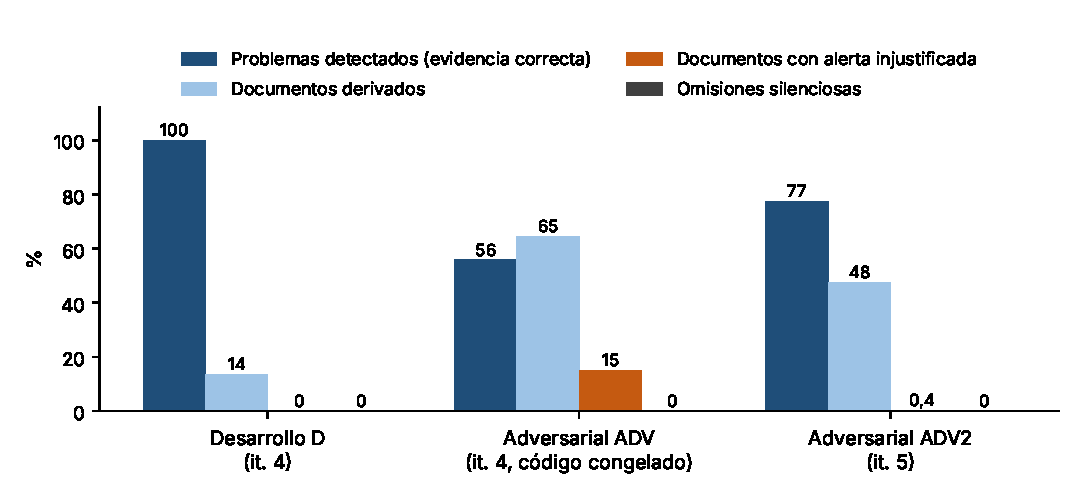
\includegraphics[width=0.92\textwidth]{fig_evaluaciones.pdf}
\caption{Indicadores principales de las tres evaluaciones. ``Problemas detectados'' se expresa sobre los problemas introducidos; los demás indicadores, sobre los documentos evaluados. Las omisiones silenciosas fueron cero en las tres. La iteración 5 sobre D dio resultados idénticos a la iteración 4.}
\label{fig:evaluaciones}
\end{figure}

\paragraph{Corpus de desarrollo.} El sistema detectó los 108 problemas introducidos (límite inferior unilateral al 95\,\%: 97,3\,\%) y no emitió alertas injustificadas. Como la mitad de prueba se observó durante el desarrollo, este resultado verifica el funcionamiento, pero no es una medición fuera de muestra. De los 24 documentos derivados, 23 correspondían a casos introducidos para ser derivados (13 nombres casi iguales, 6 firmas de un prestador no acreditado y 4 documentos en criollo) y solo uno, un código QR que no se pudo leer, a incertidumbre de lectura. Todos los campos aceptados eran correctos, pero el criterio RNF-04 no queda demostrado: en español, el límite inferior unilateral es de 98,4\,\% porque la muestra (186 campos) es menor que los 299 necesarios, y en francés es de 89,9\,\% con solo 28 campos.

\paragraph{Detección por tipo de problema.} La Tabla~\ref{tab:deteccion} desglosa la detección. El total agregado mezcla problemas que dependen de leer el contenido del documento con otros que se detectan por la firma o por el emisor, y los primeros son los más sensibles a la variación: con el código congelado sobre ADV se detectó con evidencia correcta el 42\,\% de los que dependen de la lectura, frente al 80\,\% de los demás; en ADV2, el 73\,\% y el 85\,\%. En ADV, 16 de las 96 detecciones acertaron con evidencia incorrecta: 8 alertas de firmante distinto con el RUT del empleador sin leer, 7 alertas de nombre distinto con un texto equivocado tomado como nombre y una fecha mal leída en un certificado que sí era antiguo. En D y en ADV2 todas las detecciones tuvieron la evidencia correcta. Los documentos antiguos, el ejemplo que motiva el diseño, concentraron el mayor número de problemas no detectados: en ADV se detectaron 2 de 19 certificados de antecedentes y 3 de 12 liquidaciones con más antigüedad de la permitida, y en ADV2, 10 de 16 y 7 de 12, porque la fecha no se pudo leer o interpretar y el documento se derivó.

\CatchFileDef{\tabladeteccion}{tabla_deteccion.tex}{}
\begin{table}[!htbp]
\centering
\caption{Problemas detectados con evidencia correcta sobre problemas introducidos, por tipo de documento y de problema; entre paréntesis, las detecciones con cualquier evidencia cuando difieren. En ADV2, uno de los dos nombres casi iguales en certificados de antecedentes es un error de rótulo del generador: solo difería en una tilde, que las reglas normalizan, y el sistema acertó al no informarlo.}
\label{tab:deteccion}
\footnotesize
\begin{tabularx}{\textwidth}{L ccc}
\toprule
\textbf{Problema} & \textbf{D (it. 4 y 5)} & \textbf{ADV (it. 4)} & \textbf{ADV2 (it. 5)} \\
\midrule
\tabladeteccion
\bottomrule
\end{tabularx}
\end{table}

\subsection{Evaluación adversarial del código congelado}
\label{sec:adversarial}
El corpus adversarial cambió el panorama (Tabla~\ref{tab:condiciones}). La propiedad central del diseño se mantuvo: ningún documento con un problema quedó prevalidado. Los 47 problemas que no generaron su alerta estaban en 42 documentos, y los 42 fueron derivados a revisión humana; otros 16 problemas sí generaron su alerta, pero con evidencia incorrecta (sección~\ref{sec:resultados}). Pero el código congelado emitió alertas injustificadas en 37 documentos (15\,\%), tres veces el máximo de RNF-06, y derivó el 65\,\% de los documentos.

\CatchFileDef{\tablacondiciones}{tabla_condiciones.tex}{}
\begin{table}[!htbp]
\centering
\caption{Resultados por condición en los corpus adversariales: documentos con la condición (n), derivados (Der.) y con al menos una alerta injustificada (Inj.), con el código congelado (ADV) y con la iteración 5 (ADV2). Un documento puede tener varias condiciones (por ejemplo, una diagramación y un formato de fecha).}
\label{tab:condiciones}
\footnotesize
\begin{tabularx}{\textwidth}{L rrr rrr}
\toprule
 & \multicolumn{3}{c}{\textbf{ADV (it. 4)}} & \multicolumn{3}{c}{\textbf{ADV2 (it. 5)}} \\
\cmidrule(lr){2-4}\cmidrule(lr){5-7}
\textbf{Condición} & \textbf{n} & \textbf{Der.} & \textbf{Inj.} & \textbf{n} & \textbf{Der.} & \textbf{Inj.} \\
\midrule
\tablacondiciones
\bottomrule
\end{tabularx}
\end{table}

De los 37 documentos con alertas injustificadas, 33 se debieron a defectos de lógica, no de lectura:
\begin{itemize}
  \item \textbf{Etiquetas que coincidían con otras (21 certificados).} La búsqueda de la etiqueta francesa ``Nom'' coincidía con el comienzo de ``NOMBRE'', y la etiqueta ``Nombre'' coincidía con ``Nombre del padre''. El sistema tomaba entonces un texto equivocado como nombre del titular y alertaba que no coincidía con el declarado: así ocurrió en 13 de los 17 certificados con el valor en la línea siguiente a la etiqueta y en 8 de los 12 con la trampa del nombre del padre. La Tabla~\ref{tab:condiciones} cuenta un documento más en cada grupo, cuya alerta injustificada se debió a la apostilla, como se describe más abajo.
  \item \textbf{Valores vacíos tratados como leídos (9 liquidaciones).} En el texto del PDF de las liquidaciones, cada etiqueta queda en una línea y su valor en la siguiente. El código congelado tomaba como valor el resto vacío de la línea de la etiqueta y lo comparaba como si se hubiera leído: así alertó que el nombre no coincidía en las 9 liquidaciones con la plantilla conocida cuyo texto se tomó del PDF firmado.
  \item \textbf{Una lectura faltante tratada como discrepancia (8 liquidaciones, 3 de ellas no incluidas en el punto anterior).} Cuando el RUT del empleador quedaba vacío o no se encontraba, la regla de firma lo trataba como distinto del RUT del firmante y alertaba que la firma no correspondía al empleador. Por eso ninguna de las 8 liquidaciones con firma válida se clasificó correctamente, en contra del principio de derivar ante la duda; cinco de ellas tenían además la alerta de nombre del punto anterior.
\end{itemize}

Los otros cuatro documentos tuvieron causas de lectura o de reglas incompletas. En dos certificados, el OCR deformó la leyenda de la apostilla (``dela Haye'', ``APOST, ILLE'') y el sistema alertó que faltaba; lo mismo ocurrió (``APOSTIL LE'') en un tercero, ya contado entre los anteriores por su alerta de nombre. En un pasaporte haitiano, la MRZ truncó el nombre ``Guerline'' como ``GUERL'' y el nombre declarado omitía un segundo nombre: la regla solo admite el prefijo truncado cuando la MRZ no tiene más palabras que el nombre declarado, por lo que comparó ``GUERL'' con ``GUERLINE'' y alertó. En un certificado haitiano, el nombre declarado tenía dos palabras unidas por un error de tipeo (``JeanmBaptiste'' en lugar de ``Jean-Baptiste''), y la comparación por palabras lo trató como el nombre de otra persona aun con una lectura perfecta. Estos dos últimos defectos de las reglas se identificaron al revisar los resultados después de la iteración 5, no se corrigieron y siguen presentes en el código evaluado.

Las derivaciones, en cambio, respondieron sobre todo a condiciones que el sistema no conocía, y en esos casos derivar es el comportamiento correcto: los 21 pasaportes fotografiados con márgenes no se leyeron porque la MRZ se buscaba solo en la franja inferior; las fechas con año de dos dígitos, con coma o con el mes antes del día no se pudieron interpretar; y las etiquetas no previstas impidieron reconocer los campos. La lectura de campos también se deterioró: en español, solo el 76,6\,\% de los campos aceptados era correcto, porque las etiquetas coincidentes hacían aceptar textos equivocados con confianza alta.

\paragraph{Iteración 5 sobre ADV2.} Corregidos esos defectos, las alertas injustificadas bajaron a un documento de 246 y la derivación al 48\,\%, sin omisiones silenciosas. La alerta injustificada restante se debió al mismo tipo de error de lectura de la apostilla observado en ADV, un espaciado alterado por el OCR (``deLa Haya'') que impidió detectarla; la comparación del texto sin espacios lo resolvería, pero no se incorporó para no modificar el código evaluado. Los 32 problemas no detectados, en 30 documentos, quedaron todos en documentos derivados, y uno de ellos es el error de rótulo señalado en la Tabla~\ref{tab:deteccion}; el grupo más numeroso (13) fue el de documentos con más antigüedad de la permitida cuya fecha no se pudo leer o interpretar. Las condiciones no corregidas a propósito se siguieron derivando completas: los 14 certificados con las etiquetas ``Titular'' y ``Expedido el'', los 11 con ``Lugar y fecha'', las fechas con año de dos dígitos y las 24 liquidaciones con la plantilla nueva. Como ADV2 proviene del mismo generador que motivó las correcciones, estas cifras muestran que las correcciones se generalizan a nuevas instancias de las mismas condiciones, no a condiciones nuevas.

\paragraph{Derivación por degradación de la imagen.}\label{sec:degradacion} En ADV, la derivación fue de 52\,\% en imágenes limpias, 61\,\% en fotocopias, 67\,\% con sombra y 79\,\% en fotografías de celular con fuerte degradación; en ADV2, de 32\,\%, 31\,\%, 49\,\% y 77\,\%, respectivamente (alrededor de 61 documentos por condición).

\subsection{Lectura de campos}
\label{sec:lectura}
En ADV2, la precisión de los campos aceptados en español fue de 97,9\,\% en versión estricta y de 99,3\,\% en versión funcional, con una cobertura de 52\,\%. Los tres errores estrictos aceptados fueron dos pérdidas de diacríticos (``Muñoz'' leído ``Munoz'' y ``Ñuflo'' leído ``NUFLO''), que no afectan a las reglas porque estas normalizan tildes y la Ñ, y un error de lectura (``Castañeda'' leído ``Castafieda''), que la comparación clasificó como casi igual y derivó. En francés, el único error aceptado fue un certificado con ``Nom'' y ``Prénom(s)'' en líneas separadas, del que se leyó solo el apellido; la comparación también lo derivó. Ningún error de lectura aceptado produjo una alerta. El límite inferior de la precisión (94,6\,\% en español y 79,3\,\% en francés) sigue lejos del 99\,\% exigido por RNF-04, y la cobertura muestra que, ante diagramaciones variadas, cerca de la mitad de los campos no se lee con confianza.

La confianza del OCR, además, distinguió mal los errores. En la mitad de calibración de ADV, la precisión de lo aceptado en español fue de 73\,\% sin umbral, 72\,\% con 0,80 y 63\,\% con 0,95: subir el umbral redujo la cobertura sin mejorar la precisión. En ADV2 se mantuvo entre 97 y 98,5\,\% hasta el umbral de 0,95 y llegó a 100\,\% solo con 0,96, aceptando el 24\,\% de los campos. Las abstenciones útiles vinieron sobre todo de señales estructurales (una etiqueta no encontrada, una fecha no interpretable, un dígito de control), no del umbral, de modo que el mecanismo de calibración del diseño inicial del principio 3 no quedó respaldado.

\subsection{Pasaportes, firma, QR, latencia y bitácora}
\paragraph{Pasaportes.} En ADV2 se validaron 66 de 80 MRZ: todas las de imágenes limpias y con sombra (20/20 en cada condición), 17/20 de fotocopias y 9/20 de fotografías de celular con fuerte degradación. En las 66 el número de pasaporte coincidió con la verdad. En cuatro el nombre estaba truncado, como prevé el estándar: en tres la comparación lo aceptó como prefijo, y en el cuarto, cuyo nombre declarado omitía un segundo nombre, la limitación de la regla descrita en la sección~\ref{sec:adversarial} hizo que se derivara. En dos el OCR leyó la primera letra del nombre como dígito (``J'' como ``9'' o ``4''), un error que el dígito de control no detecta y que la comparación de nombres derivó. En ADV, con el código congelado, se validaron 49 de 80, también con todos los números correctos.

\paragraph{Firma electrónica.} En ADV2 se clasificaron correctamente las 8 liquidaciones de cada variante (válida, alterada, con contenido agregado, no acreditada y sin firma), lo que respalda la vía de firma frente al OCR dentro de los límites que se discuten en la sección~\ref{sec:limfirma}. En la plantilla nueva, sin embargo, el RUT del empleador no se pudo leer: las cuatro liquidaciones con firma válida que la usaban se derivaron, y también las cuatro firmadas por otro empleador, que se derivaron en vez de alertar.

\paragraph{Códigos QR.} Se leyeron 25 de 30 códigos en ADV2 y 27 de 30 en ADV; los no leídos se derivaron. En ADV2, los cinco no leídos eran de 110 o 140 píxeles, y cuatro de ellos estaban en fotografías con fuerte degradación.

\paragraph{Latencia.} La mediana se mantuvo entre 1,26 y 1,38 segundos por documento. En ADV2 el percentil 95 subió a 5,8 segundos porque, cuando la MRZ no aparece en la franja inferior, se lee la imagen completa. Ambos valores están dentro de la meta de RNF-02, aunque se midieron sin red ni concurrencia.

\paragraph{Bitácora.} En todas las evaluaciones, la verificación contra el ancla confirmó la integridad de la bitácora y detectó la eliminación del último evento, que la sola cadena de hashes no detecta.

\subsection{Equidad por nacionalidad}
\label{sec:equidad}
La Figura~\ref{fig:pais} muestra, por país, la proporción de documentos derivados por incertidumbre de lectura, excluidos los documentos en criollo, cuya derivación es el comportamiento esperado. En el corpus de desarrollo no hubo derivaciones por incertidumbre en ningún país. En ADV2 la proporción varió entre 31\,\% (Bolivia) y 53\,\% (Venezuela), con Haití en 47\,\%. Con 32 documentos por país, los intervalos de confianza se superponen ampliamente: las diferencias entre países no son significativas (chi cuadrado, $p$ = 0,28 en ADV y 0,38 en ADV2), pero solo una diferencia de unos 35 puntos se detectaría con una potencia del 80\,\%. Además, en los generadores la nacionalidad cambia los nombres y el idioma, pero no la diagramación oficial de cada país, que es la principal fuente de variación real. Por ambas razones, la ausencia de diferencias significativas en estos corpus no demuestra la equidad: no hay evidencia de concentración de errores, pero el diseño de la evaluación no permite descartarla. Las alertas injustificadas de ADV se distribuyeron entre los cinco países (entre 3 y 6 documentos por país), y la única de ADV2 correspondió a un certificado boliviano. En francés, la precisión de lo aceptado en ADV2 (95,2\,\%) fue algo menor que en español (97,9\,\%), con una muestra de solo 21 campos. En el corpus con muestra planificada (sección~\ref{sec:muestra}), en cambio, apareció una diferencia por nacionalidad con una causa identificada: un error concreto de lectura.

\begin{figure}[!htbp]
\centering
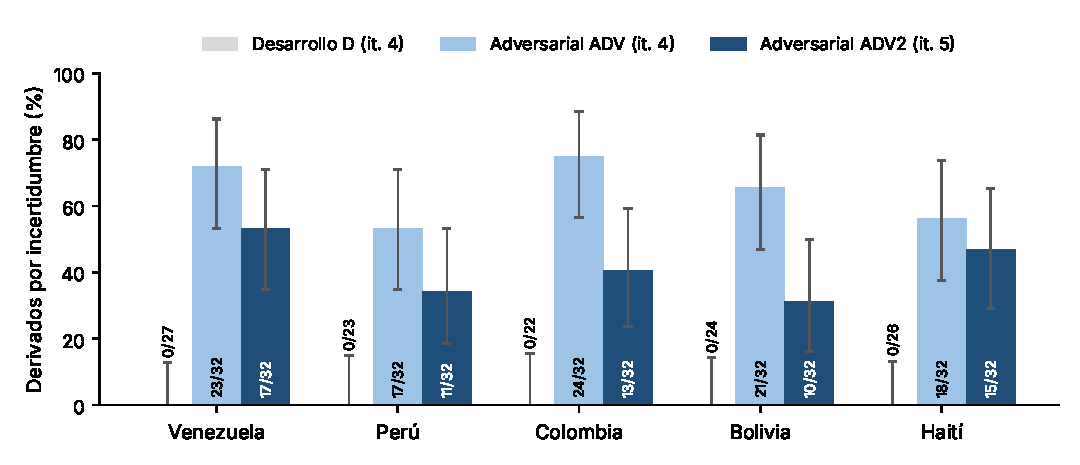
\includegraphics[width=0.92\textwidth]{fig_derivacion_pais.pdf}
\caption{Documentos derivados por incertidumbre de lectura, por país y evaluación, excluidos los documentos en criollo. Las barras de error son intervalos de Clopper-Pearson al 95\,\%; las etiquetas indican documentos derivados sobre documentos del país.}
\label{fig:pais}
\end{figure}

\subsection{Precisión con una muestra planificada}
\label{sec:muestra}
Como las muestras de D eran demasiado pequeñas para demostrar RNF-04, después de la iteración 5 se generó un corpus nuevo (P) con el generador de desarrollo, una semilla nueva (20261025) y una muestra planificada: 180 certificados de antecedentes en español (45 por país), 170 haitianos en francés y 60 liquidaciones, 410 documentos en total, evaluados completos con el código de la iteración 5 sin modificarlo. Es una medición fuera de muestra, pero en condiciones de desarrollo, no adversariales.

Con 537 campos aceptados en español y 329 en francés, la precisión alcanza la meta de RNF-04 en francés (329 de 329 correctos; límite inferior unilateral de 99,1\,\%) y, en español, solo en la versión funcional (536 de 537; límite inferior de 99,1\,\%): en la versión estricta, tres errores, dos tildes leídas con otra orientación (``Nadége'' por ``Nadège'') y una I leída como l, dejan el límite en 98,6\,\%. La cobertura de campos fue de 99\,\% en español y 97\,\% en francés. El sistema detectó con evidencia correcta 246 de 251 problemas, no tuvo omisiones silenciosas (0 de 196 documentos con problema; cota superior de 1,5\,\%), emitió una alerta injustificada en 1 de 410 documentos, por el defecto conocido de los nombres con palabras unidas, y derivó el 11\,\%.

La medición reveló, además, un error sistemático ligado al idioma. En los 11 certificados haitianos cuya fecha usaba el ordinal francés ``1er'' (los otros dos fechados el día 1 usaban el formato numérico), el OCR lo leyó como ``ler'', la fecha no se pudo interpretar y el documento se derivó. Por esa causa, la derivación por incertidumbre de lectura fue de 6,5\,\% en los certificados haitianos (11 de 170), frente a 1,7\,\% en los de los demás países (3 de 180; prueba exacta de Fisher, $p$ = 0,03). Esa agrupación se eligió después de ver los datos; la prueba entre los cinco países queda en el límite (chi cuadrado, $p$ = 0,06). El error es seguro, porque deriva y no alerta, pero su costo recae en una nacionalidad. Corregirlo es simple (aceptar ``ler'' como ``1er''), pero no se incorporó para no modificar el código evaluado. Es el tipo de hallazgo que justifica medir por nacionalidad, como propone el principio 3.

\subsection{Comparación con la línea base}
\label{sec:lineabase}
La Tabla~\ref{tab:lineabase} compara el sistema con la alternativa de derivar todo, que equivale al proceso actual de revisión manual completa. Derivar todo cumple trivialmente la seguridad y RNF-06, por lo que el aporte del sistema se mide por lo que agrega: documentos que no requieren revisión completa y problemas informados de inmediato con evidencia correcta. Con el código congelado en ADV, ese aporte fue de 35\,\% y 56\,\%, a costa de un 15\,\% de documentos con alerta injustificada; en ADV2, de 52\,\% y 77\,\%, con 0,4\,\%. La segunda fila incluye problemas cuyo resultado esperado era una derivación, que el sistema informa con su causa, pero que igualmente requieren revisión; contando solo los problemas que debían generar una alerta, el sistema informó 59 de 116 en ADV (51\,\%) y 87 de 117 en ADV2 (74\,\%).

\CatchFileDef{\tablalineabase}{tabla_linea_base.tex}{}
\begin{table}[!htbp]
\centering
\caption{El sistema frente a la línea base de derivar todo a revisión humana.}
\label{tab:lineabase}
\footnotesize
\begin{tabularx}{\textwidth}{L cccc}
\toprule
\textbf{Indicador} & \textbf{D (it. 4 y 5)} & \textbf{ADV (it. 4)} & \textbf{ADV2 (it. 5)} & \textbf{Derivar todo} \\
\midrule
\tablalineabase
\bottomrule
\end{tabularx}
\end{table}

\subsection{Amenazas a la validez de las pruebas}
\begin{itemize}
  \item \textbf{Validez externa}: todos los documentos son sintéticos. El corpus adversarial agrega variabilidad, pero los documentos reales presentan diagramaciones oficiales, fondos de seguridad, sellos y escrituras que ningún generador reproduce. Los resultados deben leerse como evidencia del comportamiento del diseño ante variaciones, no como estimación del desempeño en producción.
  \item \textbf{Generador y sistema del mismo equipo}: el corpus adversarial se escribió después del congelamiento y no se usó para ajustar el código evaluado en él, pero lo escribió quien conocía el sistema, por lo que sus condiciones reflejan variaciones anticipadas, no la distribución real. Más aún, el sistema y los generadores, incluido el adversarial, se programaron con el mismo asistente de IA (ver la declaración final), lo que reduce la independencia del corpus adversarial más de lo que sugiere el congelamiento. ADV2 comparte generador con ADV y no es independiente de las correcciones de la iteración 5.
  \item \textbf{Tamaño muestral}: en D, ADV y ADV2 la muestra en francés es pequeña (21 a 32 campos; en P, 329), hay 32 documentos por país en los corpus adversariales y algunos problemas tienen pocos casos, como los códigos QR de otra persona.
  \item \textbf{Motor y umbral}: solo se evaluó Tesseract, con un umbral fijo de 0,80 no calibrado; los resultados no se extienden a los motores en la nube.
  \item \textbf{Alcance de las métricas de lectura}: se miden solo los campos que usan las reglas, leídos por OCR desde la imagen de todos los documentos. En las liquidaciones con firma válida el sistema usa el texto del PDF firmado, de modo que para ellas la métrica mide la lectura de la imagen y no lo que efectivamente usan las reglas.
  \item \textbf{Problemas introducidos y modos de falla}: los corpus introducen justamente los problemas que las reglas buscan. No incluyen modos realistas de omisión silenciosa, como un documento con varias fechas (nacimiento, emisión, apostilla) del que se extrae la equivocada con confianza alta, o un pariente cuyo nombre contiene al declarado y que la comparación acepta como subconjunto. La regla de número de pasaporte distinto del declarado no se evaluó, porque ningún corpus introdujo ese caso. Hay al menos un modo de omisión silenciosa conocido: el intérprete de fechas convierte ``1º de agosto'' en el 10 de agosto, porque normaliza la ``º'' como ``o'' y luego la reemplaza por cero; un certificado emitido un día 1 que excediera la antigüedad máxima por menos de nueve días quedaría prevalidado sin hallazgos. Ningún corpus contiene ese formato, frecuente en documentos en español.
  \item \textbf{Construcción de los casos}: el generador de nombres de otra persona exige que todas las palabras difieran en más de dos caracteres, justo por encima del umbral de la comparación, y el generador adversarial reutiliza los generadores de nombres y la infraestructura de firma del corpus de desarrollo. Cerca de la mitad de los documentos tiene algún problema introducido, una prevalencia que no es la de expedientes reales.
  \item \textbf{Independencia de las observaciones}: los intervalos de Clopper-Pearson suponen documentos independientes, pero los errores se agrupan por plantilla y condición (por ejemplo, 14 de los 37 documentos con alerta injustificada de ADV tenían una misma diagramación), por lo que los intervalos reales son más amplios; lo mismo vale para la cota superior de las omisiones silenciosas.
  \item \textbf{Tipografía de la MRZ}: los corpus adversariales usan la misma fuente OCR-B digital que el de desarrollo, por lo que la lectura de pasaportes en imágenes limpias puede seguir siendo optimista frente a pasaportes impresos reales.
  \item \textbf{Emisor y firma simulados}: el principio 1 se evaluó con un emisor y una infraestructura de firma simulados (sección~\ref{sec:limfirma}).
\end{itemize}

\section{Especificaciones complementarias del diseño y de la maqueta}
\label{sec:anexob}
Este anexo reúne las tablas de detalle del diseño (sección~\ref{sec:diseno}) y de la maqueta (sección~\ref{sec:implementacion}).

\begin{table}[!htbp]
\centering
\caption{Requerimientos funcionales.}
\label{tab:rf}
\small
\begin{tabularx}{\textwidth}{>{\raggedright\arraybackslash}p{1.3cm} L >{\raggedright\arraybackslash}p{4.8cm}}
\toprule
\textbf{ID} & \textbf{Requerimiento} & \textbf{Criterio de aceptación} \\
\midrule
RF-01 & Autenticar a solicitantes y funcionarios & ClaveÚnica y credencial institucional \\
RF-02 & Validar formato, tamaño y resolución de cada archivo & Solo pide una nueva imagen; nunca rechaza la solicitud \\
RF-03 & Clasificar el documento según tipo y origen & Ruta asignada según la Tabla~\ref{tab:requisitos} \\
RF-04 & Obtener directamente los documentos públicos chilenos disponibles por interoperabilidad & La persona no los carga; si el emisor no responde, se le pide cargarlos \\
RF-05 & Verificar códigos de verificación y códigos QR con el emisor & Resultado registrado en el expediente \\
RF-06 & Validar la firma electrónica avanzada de documentos PDF & Integridad, ausencia de cambios posteriores a la firma, confianza del certificado y correspondencia del firmante, registrados \\
RF-07 & Extraer campos mediante OCR con nivel de confianza & Campo, valor, confianza y ubicación \\
RF-08 & Aplicar reglas de prevalidación configurables & Reglas, plazos, autenticación y excepciones por país modificables sin cambiar el código \\
RF-09 & Informar de inmediato los resultados al solicitante & Mensaje comprensible; el envío nunca se bloquea \\
RF-10 & Presentar al funcionario el expediente prevalidado & Original junto a datos extraídos, reglas, alertas y controles del expediente \\
RF-11 & Permitir al funcionario corregir cualquier dato & Corrección registrada con autor y fecha \\
RF-12 & Registrar todos los eventos del expediente & Bitácora que permite detectar alteraciones, incluida la eliminación de eventos \\
\bottomrule
\end{tabularx}
\end{table}

\begin{table}[!htbp]
\centering
\caption{Comparación documental de motores OCR. ``No verificado'': información no confirmada en fuentes oficiales durante este trabajo.}
\label{tab:matriz}
\scriptsize
\begin{tabularx}{\textwidth}{>{\raggedright\arraybackslash}p{2.7cm} L L L L}
\toprule
\textbf{Criterio} & \textbf{Amazon Textract} & \textbf{Azure AI Document Intelligence} & \textbf{Google Document AI} & \textbf{Tesseract (local)} \\
\midrule
Texto impreso en español y francés & Sí, 6 idiomas \cite{awsfaq} & Sí & Sí & Sí; evaluado en este trabajo \\
Manuscrito en español & No, solo inglés \cite{awsfaq} & No verificado & No verificado & Limitado \\
Lectura nativa de pasaportes de cualquier país & No; API orientada a documentos de EE.\,UU. \cite{awsid} & Sí, incluida la MRZ \cite{azureid} & No confirmado; el anuncio de 2022 incluía pasaportes de EE.\,UU. \cite{googleid} & No; requiere un modelo para OCR-B \cite{doubango} y la validación de la MRZ, implementada en la maqueta \\
Evidencia de precisión & Alta en inglés \cite{hegghammer2022} & No evaluado en \cite{hegghammer2022} & La mejor en inglés \cite{hegghammer2022} & Probado en la maqueta con documentos ficticios (Anexo~\ref{sec:anexo}) \\
Procesamiento en Chile hoy & No; sin región en Sudamérica \cite{awsendpoints}; región Chile anunciada \cite{awschile} & Región Chile Central desde 2025 \cite{mschile}; disponibilidad del servicio no verificada & No; sin región en Sudamérica \cite{gdocairegions} & Sí \\
Precio por página de formularios & USD 0,05 \cite{awspricing} & No verificado en la fuente oficial & USD 0,03 \cite{googlepricing} & Sin costo de licencia \\
Retención de datos & Exclusión del entrenamiento mediante política \cite{awsoptout} & Borrado a las 24 horas \cite{azureprivacy} & No verificado & Sin terceros \\
\bottomrule
\end{tabularx}
\end{table}

\subsection{Módulos de la maqueta}
\begin{itemize}
  \item \textbf{Adaptador OCR} (\texttt{ocr.py}): define una interfaz común que devuelve líneas con texto y confianza. Para pasaportes, Tesseract lee la franja inferior con el modelo para OCR-B y el alfabeto restringido a la MRZ, en dos escalas; si no encuentra una MRZ con dígitos de control válidos, lee la imagen completa, lo que cubre fotografías en que el pasaporte no ocupa toda la imagen. Los adaptadores de Textract y Azure implementan la misma interfaz.
  \item \textbf{Preprocesamiento} (\texttt{preproceso.py}): estima la inclinación maximizando la varianza del perfil de proyección horizontal y corrige la iluminación dividiendo por el fondo estimado.
  \item \textbf{MRZ} (\texttt{mrz.py}): interpreta la MRZ, valida sus cinco dígitos de control, corrige las confusiones habituales según la posición (letras por dígitos en campos numéricos y viceversa en nombres y códigos de país), repara la inserción de un carácter espurio solo si existe una única variante que valida los cinco dígitos y detecta los nombres truncados.
  \item \textbf{Extracción} (\texttt{extraccion.py}): ubica los campos por sus etiquetas en español y francés, exigiendo que la etiqueta termine en un límite de palabra y vaya seguida de un separador, y admite el valor en la línea siguiente; interpreta fechas numéricas y textuales en ambos idiomas; compara nombres; y detecta apostillas y legalizaciones.
  \item \textbf{Reglas} (\texttt{reglas.py} y \texttt{reglas.yaml}): implementa las reglas de la sección~\ref{sec:reglas}.
  \item \textbf{Verificación} (\texttt{verificacion.py}): decodifica códigos QR y los consulta al emisor (simulado en la maqueta), y valida firmas electrónicas con pyHanko: integridad, nivel de modificación posterior a la firma, cadena de certificación hasta las raíces de prestadores acreditados y RUT del firmante.
  \item \textbf{Bitácora} (\texttt{bitacora.py}): cada evento incluye el hash del anterior, de modo que modificar un evento rompe la cadena. Como eliminar los últimos eventos o reescribir toda la cadena no la rompe, la bitácora emite además un \emph{ancla}, con el número de eventos y el hash final autenticados con una clave externa, que en producción se custodiaría fuera del sistema; la verificación contra el ancla detecta también esas alteraciones.
  \item \textbf{Orquestación y API} (\texttt{pipeline.py}, \texttt{api.py}): procesan cada documento por su vía, responden al solicitante con los mensajes y siempre permiten el envío, aplican los controles a nivel de expediente y exponen al funcionario los datos, los hallazgos y el estado de la bitácora.
\end{itemize}

El Listado~\ref{lst:respuesta} muestra respuestas reales de la API, ejecutada sobre documentos ficticios: un pasaporte vencido, una liquidación de sueldo a la que se agregó contenido después de firmada y un certificado de antecedentes con una fecha de año con dos dígitos, que se deriva en vez de alertar.

\begin{lstlisting}[caption={Respuestas de la API de la maqueta al solicitante (documentos ficticios).},label={lst:respuesta},captionpos=b]
POST /solicitudes/{id}/documentos  (tipo=pasaporte, pais=VEN)
{"estado": "CON_ALERTAS", "via": "ocr_mrz",
 "mensajes": ["El pasaporte está vencido"], "puede_enviar": true}

POST /solicitudes/{id}/documentos  (tipo=liquidacion, con PDF firmado)
{"estado": "CON_ALERTAS", "via": "firma_y_ocr",
 "mensajes": ["Se agregó contenido después de la firma"], "puede_enviar": true}

POST /solicitudes/{id}/documentos  (tipo=antecedentes_extranjero, pais=VEN)
{"estado": "REVISION_HUMANA", "via": "ocr",
 "mensajes": ["No se pudo interpretar la fecha '15/08/26'"], "puede_enviar": true}
\end{lstlisting}

\begin{table}[!htbp]
\centering
\caption{Tecnologías de la maqueta.}
\label{tab:stack}
\small
\begin{tabularx}{\textwidth}{>{\raggedright\arraybackslash}p{3.4cm} >{\raggedright\arraybackslash}p{4.6cm} L}
\toprule
\textbf{Función} & \textbf{Tecnología} & \textbf{Justificación} \\
\midrule
API REST & FastAPI & Tipado, documentación automática y ejecución asíncrona \\
Motor OCR local & Tesseract 5.3.4 con los modelos rápidos (\emph{tessdata\_fast}) de español, francés e inglés \cite{smith2007} & Código abierto, procesamiento en Chile y sin terceros \\
Lectura de la MRZ & Modelo de Tesseract para OCR-B de DoubangoTelecom, licencia BSD-3 \cite{doubango} & El modelo genérico confunde el relleno \texttt{<} con letras (sección~\ref{sec:mrz}) \\
Adaptadores en la nube & SDK de AWS (Textract) y de Azure (Document Intelligence) & Implementados con la misma interfaz; no ejecutados por falta de cuentas; el de Textract usa por ahora solo las líneas de texto \\
Preprocesamiento de imagen & OpenCV & Corrección de inclinación y de iluminación \\
Comparación de nombres & RapidFuzz (distancia de Levenshtein por palabra) & Tolerancia controlada a errores de uno o dos caracteres \\
Firma electrónica avanzada & pyHanko y pypdf & Integridad, cambios posteriores a la firma, cadena de certificación, RUT del firmante y texto del PDF firmado \\
Códigos QR & OpenCV & Decodificación sin dependencias externas \\
Reglas & Archivo YAML & Modificación sin cambiar el código (RF-08) \\
Bitácora & SQLite (maqueta) o PostgreSQL & Cadena de hashes SHA-256 con ancla externa autenticada (HMAC) \\
Pruebas & SciPy, Matplotlib y pytest & 40 pruebas automatizadas, intervalos de Clopper-Pearson y figuras \\
\bottomrule
\end{tabularx}
\end{table}

\begin{table}[!htbp]
\centering
\caption{Estado de implementación de los requerimientos funcionales en la maqueta.}
\label{tab:implementacion}
\small
\begin{tabularx}{\textwidth}{>{\raggedright\arraybackslash}p{1.3cm} >{\raggedright\arraybackslash}p{2.6cm} L}
\toprule
\textbf{ID} & \textbf{Estado} & \textbf{Detalle} \\
\midrule
RF-01 & No implementado & Sin ClaveÚnica ni credencial institucional; la API se usa directamente \\
RF-02 & No implementado & No se valida formato, tamaño ni resolución del archivo \\
RF-03 & No implementado & El tipo de documento y el idioma los declara quien carga el documento \\
RF-04 & No implementado & No hay obtención por interoperabilidad \\
RF-05 & Simulado & El emisor es un registro local que responde a los códigos QR \\
RF-06 & Implementado & Con los límites de la sección~\ref{sec:limfirma} \\
RF-07 & Parcial & Campo, valor y confianza, con Tesseract; la ubicación no se conserva y los adaptadores en la nube no se ejecutaron \\
RF-08 & Implementado & Reglas, plazos, autenticación y excepciones en un archivo YAML \\
RF-09 & Implementado & Respuesta inmediata de la API; el envío nunca se bloquea \\
RF-10 & Parcial & La API entrega datos, hallazgos y controles del expediente; no hay panel con el original \\
RF-11 & No implementado & No hay corrección de datos por el funcionario \\
RF-12 & Implementado & En SQLite, con la clave del ancla fija en el código \\
\bottomrule
\end{tabularx}
\end{table}

\begin{table}[!htbp]
\centering
\caption{Riesgos y estrategias de mitigación.}
\label{tab:riesgos}
\small
\begin{tabularx}{\textwidth}{>{\raggedright\arraybackslash}p{5cm} L}
\toprule
\textbf{Riesgo} & \textbf{Mitigación} \\
\midrule
Baja calidad de imagen & Preprocesamiento, control de resolución, solicitud inmediata de nueva imagen y derivación de lo que no se lee \\
Diagramaciones o etiquetas no previstas & Derivación del documento no reconocido sin alertar (observado en las pruebas de la maqueta); incorporación de etiquetas a partir de documentos reales \\
Lecturas defectuosas convertidas en alertas & Regla de derivar ante la duda; medición de alertas injustificadas en cada versión \\
Manuscritos o idiomas no soportados & Derivación directa a revisión humana sin penalizar a la persona (observado en las pruebas de la maqueta) \\
Errores de OCR concentrados en una nacionalidad & Métricas por país en cada versión y derivación de lo dudoso \\
Confusiones que el dígito de control no detecta (G y 6, nombres) & Derivación de números y nombres casi coincidentes \\
Documentos falsificados o alterados & Verificación con el emisor, validación de firma y revisión humana \\
Firma por un representante o con varios firmantes & Verificar la representación y validar todas las firmas; mientras tanto, derivar (sección~\ref{sec:limfirma}) \\
Sesgo de automatización de los funcionarios & Medición en el piloto de alertas corregidas o descartadas; capacitación \\
Uso de los documentos por el proveedor & Datos en Chile, solo imágenes al OCR, exclusión del entrenamiento \\
Dependencia de un proveedor & Adaptador OCR con interfaz común (RNF-12) \\
\bottomrule
\end{tabularx}
\end{table}

\begin{table}[!htbp]
\centering
\caption{Costo anual estimado de procesamiento OCR en la nube según páginas por solicitud (150.000 solicitudes; precios de lista de Textract \cite{awspricing}: USD 0,0015 por la página del pasaporte, precio de detección de texto, y USD 0,05 por página de formularios; todos los escenarios quedan bajo el millón de páginas mensuales).}
\label{tab:costos}
\small
\begin{tabular}{lrrr}
\toprule
\textbf{Páginas por solicitud} & \textbf{6} & \textbf{10} & \textbf{15} \\
\midrule
Páginas al mes & 75.000 & 125.000 & 187.500 \\
Costo OCR anual (USD) & 37.725 & 67.725 & 105.225 \\
Infraestructura estimada (USD) & 10.000 & 10.000 & 10.000 \\
\textbf{Costo operativo anual (USD)} & \textbf{47.725} & \textbf{77.725} & \textbf{115.225} \\
Costo por solicitud (USD) & 0,32 & 0,52 & 0,77 \\
\bottomrule
\end{tabular}
\end{table}

\end{document}
